\documentclass[18pt,xcolor=table]{beamer}

%!TEX root = ./main.tex
\usepackage {bbm}
\usepackage {textpos}
\usepackage {tikz}
\usepackage {graphicx}


\definecolor{blue1}{RGB}{176,196,222 }
\definecolor{blue2}{RGB}{54,100,139}

\definecolor{grey1}{RGB}{139,139,131}
\definecolor{grey2}{RGB}{235,235,235}

\definecolor{black1}{RGB}{50,50,50}

\mode<presentation>
{
  % \usetheme{Pittsburgh}   
  %\usetheme{Boadilla}  
\usetheme{Madrid}  
  \usefonttheme[onlymath]{serif}
  \setbeamertemplate{items}[circle] 
  \setbeamertemplate{sections/subsections in toc}[circle]
  \setbeamercovered{invisible}
  \setbeamertemplate{navigation symbols}{}
% \usecolortheme{seahorse}
%
%  % Color Theme 
  \setbeamercolor{normal text}{bg=white,fg=black1} %All standard text
  \setbeamercolor{structure}{fg=blue2} %% Table of Contents 

  \setbeamercolor*{frametitle}{fg=black1,bg=grey2} % Frame title colors
%  \setbeamerfont{frametitle}{series=\bfseries}
  \setbeamercolor*{framesubtitle}{fg=blue2} % Frame subtitle color

  \setbeamercolor*{palette primary}{use=structure,fg=black1, bg=grey2} %right bottom
  \setbeamercolor*{palette secondary}{use=structure,bg=blue1} %middle bottom
  \setbeamercolor*{palette tertiary}{use=structure,bg=blue2,fg=grey2} %left bottom

  \setbeamercolor*{block body}{fg=black1,bg=blue1!10} % Color of blocks
  \setbeamercolor*{block title}{parent=structure,fg=black1,bg=blue1} % Block Titles
  \setbeamercolor{alerted text}{fg=blue2!85!black,} % Alerted Text (ie. highlight with \alert)
  \setbeamerfont{alerted text}{series=\bfseries}

  % not sure what these do.
  \setbeamercolor{item projected}{use=item,fg=black1,bg=item.fg!35}
  \setbeamercolor*{block title alerted}{parent=alerted text,bg=black1!15}
  \setbeamercolor*{block title example}{parent=example text,bg=black1!15}
  \setbeamerfont{framesubtitle}{size=\small}
}

\makeatletter
\setbeamertemplate{footline}
{
  \leavevmode%
    \hbox{%
      \begin{beamercolorbox}[wd=.333333\paperwidth,ht=2.25ex,dp=1ex,center]{author in head/foot}%
        \usebeamerfont{author in head/foot}\insertshortauthor%~~\beamer@ifempty{\insertshortinstitute}{}{(\insertshortinstitute)}
      \end{beamercolorbox}%
        \begin{beamercolorbox}[wd=.333333\paperwidth,ht=2.25ex,dp=1ex,center]{title in head/foot}%
        \usebeamerfont{title in head/foot}\insertshorttitle
        \end{beamercolorbox}%
        \begin{beamercolorbox}[wd=.333333\paperwidth,ht=2.25ex,dp=1ex,right]{date in head/foot}%
        \usebeamerfont{date in head/foot}\insertshortdate{}\hspace*{2em}
        \insertframenumber{} / \inserttotalframenumber\hspace*{2ex} 
      \end{beamercolorbox}}%
        \vskip0pt%
}
\makeatother

%\usepackage{kerkis}
\usepackage{helvet} 
\usepackage[T1]{fontenc}
\usepackage[protrusion=true,expansion=true]{microtype}
\usepackage{amsmath}

\renewcommand*{\thefootnote}{\fnsymbol{footnote}}


\pgfdeclareimage[height=1.5cm]{logo}{./logos/hd_logo}
\pgfdeclareimage[height=0.8cm]{small_logo}{./logos/hd_logo}

\AtBeginSection[] { 
  \begin{frame}[plain] 
    \frametitle{\bf Outline:}
    \framesubtitle{~~} 
    \tableofcontents[currentsection] 
  \end{frame} 
  \addtocounter{framenumber}{-1} 
} 

\setbeamercovered{transparent}

%%%%%%%%%%%%%%%%%%%%%%%
% user-defined commands
%%%%%%%%%%%%%%%%%%%%%%%
%!TEX root = ../main.tex


\newcommand{\beq}{\begin{equation}}
\newcommand{\eeq}{\end{equation}}

\newcommand{\eq}[1]{\begin{align*}#1\end{align*}}

\newcommand{\bfi}{\begin{figure}}
\newcommand{\efi}{\end{figure}}

\newcommand{\icg}{\includegraphics}

\newcommand{\bdm}{\begin{displaymath}}
\newcommand{\edm}{\end{displaymath}}

\newcommand{\beqa}{\begin{eqnarray}}
\newcommand{\eeqa}{\end{eqnarray}}

\newcommand{\beqas}{\begin{eqnarray*}}
\newcommand{\eeqas}{\end{eqnarray*}}

\newcommand{\barr}{\begin{array}}
\newcommand{\earr}{\end{array}}

\newcommand{\bit}{\begin{itemize}}
\newcommand{\eit}{\end{itemize}}

\newcommand{\qq}[1]{\qquad \mbox{#1} \qquad}

\def\hyph{-\penalty0\hskip0pt\relax}

% Tikz
\definecolor{blue1}{RGB}{176,196,222 }
\definecolor{blue2}{RGB}{54,100,139}
\definecolor{grey1}{RGB}{139,139,131}
\definecolor{grey2}{RGB}{235,235,235}
\definecolor{black1}{RGB}{50,50,50}


%Spaces
\newcommand{\Sp}[1]{{\cal #1}}
%
\newcommand{\sA}{\Sp{A}}
\newcommand{\sB}{\Sp{B}}
\newcommand{\sC}{\Sp{C}}
\newcommand{\sD}{\Sp{D}}
\newcommand{\sE}{\Sp{E}}
\newcommand{\sF}{\Sp{F}}
\newcommand{\sG}{\Sp{G}}
\newcommand{\sH}{\Sp{H}}
\newcommand{\sI}{\Sp{I}}
\newcommand{\sJ}{\Sp{J}}
\newcommand{\sK}{\Sp{K}}
\newcommand{\sL}{\Sp{L}}
\newcommand{\sM}{\Sp{M}}
\newcommand{\sN}{\Sp{N}}
\newcommand{\sO}{\Sp{O}}
\newcommand{\sP}{\Sp{P}}
\newcommand{\sQ}{\Sp{Q}}
\newcommand{\sR}{\Sp{R}}
\newcommand{\sS}{\Sp{S}}
\newcommand{\sT}{\Sp{T}}
\newcommand{\sU}{\Sp{U}}
\newcommand{\sV}{\Sp{V}}
\newcommand{\sW}{\Sp{W}}
\newcommand{\sX}{\Sp{X}}
\newcommand{\sY}{\Sp{Y}}
\newcommand{\sZ}{\Sp{Z}}

%Vectors
\newcommand{\V}[1]{{\bf #1}}
%
\newcommand{\va}{\V{a}}
\newcommand{\vb}{\V{b}}
\newcommand{\vc}{\V{c}}
\newcommand{\vd}{\V{d}}
\newcommand{\ve}{\V{e}}
\newcommand{\vf}{\V{f}}
\newcommand{\vg}{\V{g}}
\newcommand{\vh}{\V{h}}
\newcommand{\vi}{\V{i}}
\newcommand{\vj}{\V{j}}
\newcommand{\vk}{\V{k}}
\newcommand{\vl}{\V{l}}
\newcommand{\vm}{\V{m}}
\newcommand{\vn}{\V{n}}
\newcommand{\vo}{\V{o}}
\newcommand{\vp}{\V{p}}
\newcommand{\vq}{\V{q}}
\newcommand{\vr}{\V{r}}
\newcommand{\vs}{\V{s}}
\newcommand{\vt}{\V{t}}
\newcommand{\vu}{\V{u}}
\newcommand{\vv}{\V{v}}
\newcommand{\vw}{\V{w}}
\newcommand{\vx}{\V{x}}
\newcommand{\vy}{\V{y}}
\newcommand{\vz}{\V{z}}

\newcommand{\vA}{\V{A}}
\newcommand{\vB}{\V{B}}
\newcommand{\vC}{\V{C}}
\newcommand{\vD}{\V{D}}
\newcommand{\vE}{\V{E}}
\newcommand{\vF}{\V{F}}
\newcommand{\vG}{\V{G}}
\newcommand{\vH}{\V{H}}
\newcommand{\vI}{\V{I}}
\newcommand{\vJ}{\V{J}}
\newcommand{\vK}{\V{K}}
\newcommand{\vL}{\V{L}}
\newcommand{\vM}{\V{M}}
\newcommand{\vN}{\V{N}}
\newcommand{\vO}{\V{O}}
\newcommand{\vP}{\V{P}}
\newcommand{\vQ}{\V{Q}}
\newcommand{\vR}{\V{R}}
\newcommand{\vS}{\V{S}}
\newcommand{\vT}{\V{T}}
\newcommand{\vU}{\V{U}}
\newcommand{\vV}{\V{V}}
\newcommand{\vW}{\V{W}}
\newcommand{\vX}{\V{X}}
\newcommand{\vY}{\V{Y}}
\newcommand{\vZ}{\V{Z}}

\newcommand{\vone}{\V{1}}
\newcommand{\vzero}{\V{0}}
\newcommand{\B}{\V{B}}
\newcommand{\E}{\V{E}}
\newcommand{\Er}{\V{E}_r}
\newcommand{\Es}{\V{E}_s}
\newcommand{\un}{\hat{\vn}}



%Vectors
\newcommand{\T}[1]{\underline{\bf #1}}
%
\newcommand{\ta}{\T{a}}
\newcommand{\tb}{\T{b}}
\newcommand{\tc}{\T{c}}
%\newcommand{\td}{\T{d}}
\newcommand{\te}{\T{e}}
\newcommand{\tf}{\T{f}}
\newcommand{\tg}{\T{g}}
%\newcommand{\th}{\T{h}}
\newcommand{\ti}{\T{i}}
\newcommand{\tj}{\T{j}}
\newcommand{\tk}{\T{k}}
\newcommand{\tl}{\T{l}}
\newcommand{\tm}{\T{m}}
\newcommand{\tn}{\T{n}}
%\newcommand{\to}{\T{o}}
\newcommand{\tp}{\T{p}}
\newcommand{\tq}{\T{q}}
\newcommand{\tr}{\T{r}}
\newcommand{\ts}{\T{s}}
%\newcommand{\tt}{\T{t}}
\newcommand{\tu}{\T{u}}
\newcommand{\tv}{\T{v}}
\newcommand{\tw}{\T{w}}
\newcommand{\tx}{\T{x}}
\newcommand{\ty}{\T{y}}
\newcommand{\tz}{\T{z}}

\newcommand{\tA}{\T{A}}
\newcommand{\tB}{\T{B}}
\newcommand{\tC}{\T{C}}
\newcommand{\tD}{\T{D}}
\newcommand{\tE}{\T{E}}
\newcommand{\tF}{\T{F}}
\newcommand{\tG}{\T{G}}
\newcommand{\tH}{\T{H}}
\newcommand{\tI}{\T{I}}
\newcommand{\tJ}{\T{J}}
\newcommand{\tK}{\T{K}}
\newcommand{\tL}{\T{L}}
\newcommand{\tM}{\T{M}}
\newcommand{\tN}{\T{N}}
\newcommand{\tO}{\T{O}}
\newcommand{\tP}{\T{P}}
\newcommand{\tQ}{\T{Q}}
\newcommand{\tR}{\T{R}}
\newcommand{\tS}{\T{S}}
\newcommand{\tT}{\T{T}}
\newcommand{\tU}{\T{U}}
\newcommand{\tV}{\T{V}}
\newcommand{\tW}{\T{W}}
\newcommand{\tX}{\T{X}}
\newcommand{\tY}{\T{Y}}
\newcommand{\tZ}{\T{Z}}

\newcommand{\tone}{\T{1}}
\newcommand{\tzero}{\T{0}}

%Matrix
\newcommand{\M}[1]{{\mathbb #1}}
%
\newcommand{\mA}{\M{A}}
\newcommand{\mB}{\M{B}}
\newcommand{\mC}{\M{C}}
\newcommand{\mD}{\M{D}}
\newcommand{\mE}{\M{E}}
\newcommand{\mF}{\M{F}}
\newcommand{\mG}{\M{G}}
\newcommand{\mH}{\M{H}}
\newcommand{\mI}{\M{I}}
\newcommand{\mJ}{\M{J}}
\newcommand{\mK}{\M{K}}
\newcommand{\mL}{\M{L}}
\newcommand{\mM}{\M{M}}
\newcommand{\mN}{\M{N}}
\newcommand{\mO}{\M{O}}
\newcommand{\mP}{\M{P}}
\newcommand{\mQ}{\M{Q}}
\newcommand{\mR}{\M{R}}
\newcommand{\mS}{\M{S}}
\newcommand{\mT}{\M{T}}
\newcommand{\mU}{\M{U}}
\newcommand{\mV}{\M{V}}
\newcommand{\mW}{\M{W}}
\newcommand{\mX}{\M{X}}
\newcommand{\mY}{\M{Y}}
\newcommand{\mZ}{\M{Z}}

\newcommand{\mzero}{\M{0}}
\newcommand{\mone}{\M{1}}

% Derivatives
\newcommand{\pd}[2]{\frac{\partial #1}{\partial #2}}
\newcommand{\ppd}[2]{\frac{\partial^2 #1}{\partial #2^2}}
\newcommand{\td}[2]{\frac{\mathrm{d} #1}{\mathrm{d} #2}}

\newcommand{\px}{ \partial_{x} }
\newcommand{\py}{ \partial_{y} }
\newcommand{\pz}{ \partial_{z} }
\newcommand{\pt}{ \partial_{t} }
\newcommand{\ptt}{ \partial_{tt} }

\newcommand{\Div}[1]{\nabla \cdot #1}
\newcommand{\Curl}[1]{\nabla \times #1}
\newcommand{\Ctwo}[1]{\nabla_2 \times #1}
\newcommand{\Grad}[1]{\nabla #1}
\newcommand{\Gperp}[1]{\nabla^\perp #1}
\newcommand{\Lap}[1]{\Delta #1}

%integral d
\newcommand{\dd}[0]{\, \mathrm{d}}

% common discrete quantities
\newcommand{\dt}[0]{\delta t}

% physical variables
\newcommand{\eps}[0]{\epsilon_0}
\newcommand{\mus}[0]{\mu_0}
\newcommand{\boltz}[0]{\kappa_B}
\newcommand{\s}[0]{\alpha}
\newcommand{\vths}[0]{v_{th_\s}}
\newcommand{\vthe}[0]{v_{th_e}}
\newcommand{\vthi}[0]{v_{th_i}}
\newcommand{\Om}[0]{\Omega}
\newcommand{\bdOm}{\partial \Omega}

% bracketing
\newcommand{\inner}[2]{\langle #1, #2 \rangle}
\newcommand{\lb}[0]{\left[}
\newcommand{\rb}[0]{\right]}
\newcommand{\parn}[1]{\left( #1 \right)}
\newcommand{\la}{\langle}
\newcommand{\ra}{\rangle}
\newcommand{\lcb}{\left\{}
\newcommand{\rcb}{\right\}}

\newcommand{\mathAnd}{\,\,\mbox{and}\,\,}
\newcommand{\mathOn}{\,\,\mbox{on}\,\,}

\newcommand{\h}{\hat}
\newcommand{\wh}{\widehat}
%\newcommand{\ul}{\underline}

% math operators
\DeclareMathOperator{\Trace}{trace}
\DeclareMathOperator{\Supp}{supp}
\DeclareMathOperator{\Span}{span}
\DeclareMathOperator{\floor}{floor}
\DeclareMathOperator{\diam}{diam}
\DeclareMathOperator{\ceil}{ceil}
\DeclareMathOperator*{\argmin}{arg\,min}


\newcommand{\red}[1]{\textcolor{red}{#1}}
%added macro definitions here

\usepackage{tikz}
\usepackage{tabularx}
\usetikzlibrary{decorations.markings}
\usetikzlibrary{arrows,positioning} 

\usepackage{cancel}
\usepackage{hyperref}
\usepackage{caption}
\usepackage{subcaption}
\usepackage[]{algorithm}
\usepackage{algpseudocode}
\captionsetup{compatibility=false}


\title[Multigrid]{Introduction to Multigrid Methods}
\subtitle{Day 2: Geometric Multigrid}
\author[Mitchell]{Wayne Mitchell}
\institute{\pgfuseimage{logo}\\Universit\"at Heidelberg\\Institut f\"ur Technische Informatik}
\date[]{\alert{}}


\begin{document}
%!TEX root = ./main.tex
\tikzstyle{block} = [rectangle, draw, rounded corners, shade, top color=white, text width=5em,
  bottom color=blue!50!black!20, draw=blue!40!black!60, very thick, text centered, minimum height=4em]
  \tikzstyle{line} = [draw, -latex']
  \tikzstyle{cloud} = [draw, ellipse,top color=white, bottom color=red!20, node distance=2cm, minimum height=2em]

  \frame{\titlepage}

  \addtobeamertemplate{frametitle}{}{%
      \begin{textblock*}{100mm}(0.9\textwidth,-0.88cm)
    \pgfuseimage{small_logo}
    \end{textblock*}
  }

\AtBeginSection[] { 
  \begin{frame}[t]
    \frametitle{\bf Outline:}
    \framesubtitle{~~} 
    \tableofcontents[currentsection] 
  \end{frame} 
  \addtocounter{framenumber}{-1} 
} 

\let\tempone\itemize
\let\temptwo\enditemize
\renewenvironment{itemize}{\tempone\addtolength{\itemsep}{0.5\baselineskip}}{\temptwo}

\DeclareRobustCommand{\Chi}{\raisebox{2pt}{$\chi$}}
%%%%%%%%%%%%%%%%%%%%%%%%%%%%%%%%%%%%%%%%%%%%%%%%%%%%%%%%%%%%%%%%%%%%%%%%%%%%%%%%

% Slide
\begin{frame}{}
\begin{block}{Day 2 Goals}
\bit
\item Session 1:
\bit
\item Basic theoretical motivations for multigrid
\item Move from basic iterative methods toward multigrid
\eit
\item Session 2:
\bit
\item Define basic multgrid components: relaxation, interpolation, and restriction
\item Define multigrid cycles and examine cost and convergence
\eit
\item Session 3:
\bit
\item Discussion and hands-on examples
\eit
\eit
\end{block}
\end{frame}

% Slide
\begin{frame}{}
\begin{block}{Acknowledgements}
\bit
\item These slides are based on previous tutorials by Steve McCormick, Van Henson, Rob Falgout, Irad Yavneh, David Moulton, Luke Olson.
\item https://github.com/copper-multigrid-conference
\eit
\end{block}
\end{frame}

\begin{frame}
\frametitle{\bf Outline:}
\framesubtitle{~~}
\tableofcontents
\end{frame}

%%%%%%%%%%%%%%%%%%%%%%%%%%%%%%%%%%%%%%%%%%%%%%%%%%%%%%%%%%%%%%%%%%%%%%%%%%%%%%%%

\section{Basic iterative methods on a model problem}


% Slide
\begin{frame}{Basic iterative methods on a model problem}
\begin{block}{Moving from basic iterative methods to multigrid}
\bit
\item Focus on a model elliptic PDE problem
\item Examine the behavior of basic iterative methods on this problem
\item Use that behavior to motivate the move towards multigrid
\eit
\end{block}
\end{frame}

% Slide
\begin{frame}{Basic iterative methods on a model problem}
\begin{block}{Model problem: Poisson}
\bit
\item Classic model problem is a simple Poisson problem with zero Dirichlet boundary conditions:
\eq{
\Delta u &= f, & \Omega \\
u &= 0, & \partial \Omega
}
\item Discretizing with finite differences on a regular 1D mesh:
\eit
\eq{
&\frac{-u_{i-1} + 2u_i - u_{i+1}}{h^2} = f_i, & i = 1,2,..., N-1 \\
&u_0 = u_N = 0
}
\end{block}
\end{frame}

% Slide
\begin{frame}{Basic iterative methods on a model problem}
\begin{block}{Model problem: Poisson}
\begin{center}
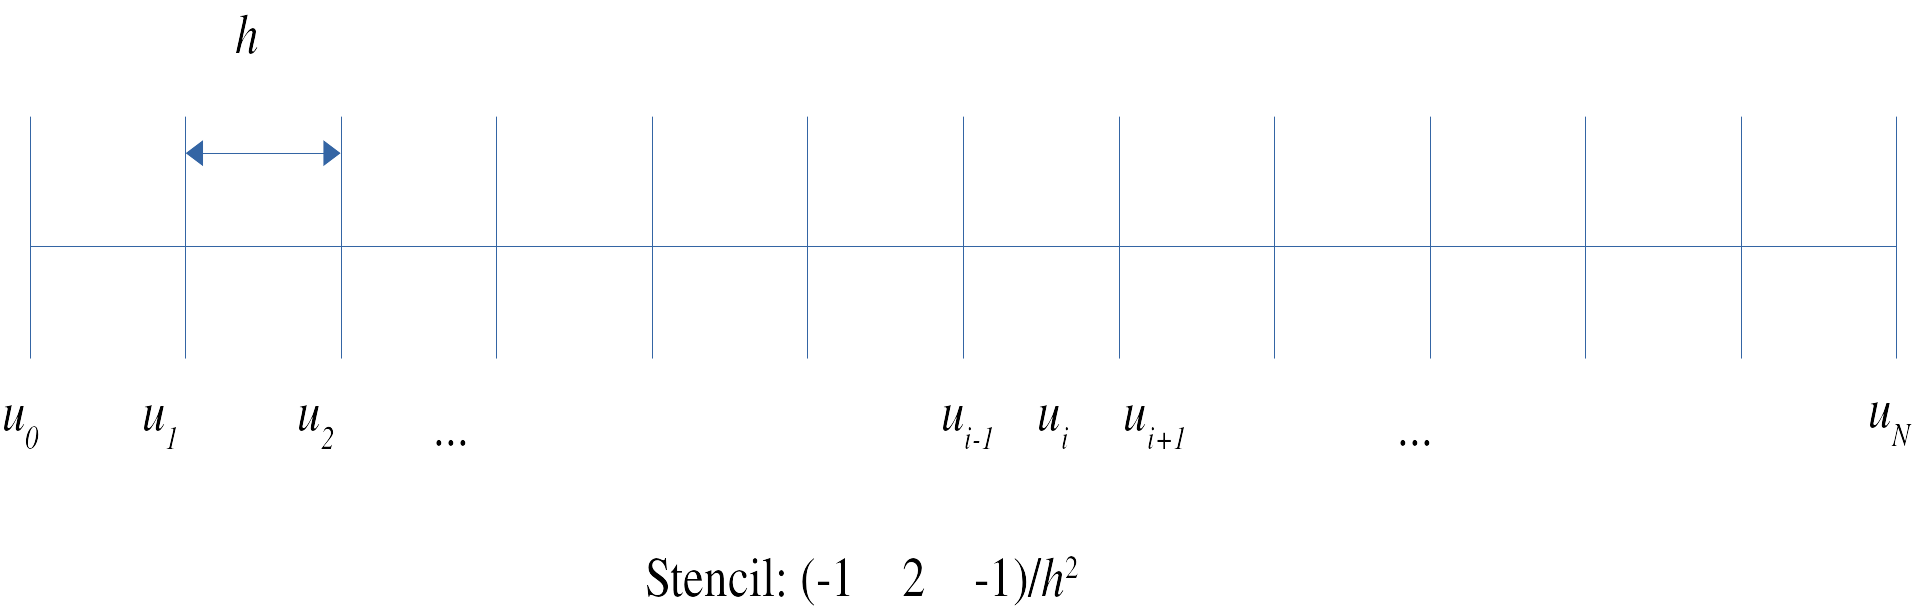
\includegraphics[width=0.7\textwidth]{../figures/1DFDPoisson}
\end{center}
\eq{
\frac{1}{h^2}\begin{bmatrix}
2 & -1 & & & & & & \\
-1 & 2 & -1 & & & & & \\
& -1 & 2 & - 1 & & & & \\
&  & \ddots & \ddots & \ddots & & & \\
& & & & & & & \\
& & & & & -1 & 2 & -1 \\
& & & & & & -1 & 2 \\
\end{bmatrix}
\begin{bmatrix}
u_1 \\
u_2 \\
\\
\vdots \\
\\
\\
u_{N-1} \\
\end{bmatrix}
=
\begin{bmatrix}
f_1 \\
f_2 \\
\\
\vdots \\
\\
\\
f_{N-1} \\
\end{bmatrix}
}
\end{block}
\end{frame}

% Slide
\begin{frame}{Basic iterative methods on a model problem}
\begin{block}{Behavior of Gauss-Seidel}
\bit
\item Gauss-Seidel as a stand-alone solver convergese very slowly
\item With a random initial guess, convergence is swift for a couple of iterations, then stalls
\eit
\end{block}
\begin{center}
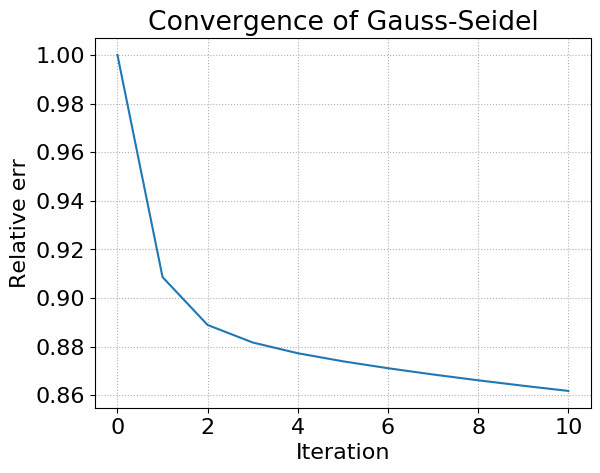
\includegraphics[width=0.5\textwidth]{../figures/gaussSeidelConvRand}
\end{center}
\end{frame}

% Slide
\begin{frame}{Basic iterative methods on a model problem}
\begin{block}{Behavior of Gauss-Seidel}
\bit
\item Gauss-Seidel seems to "smooth out" the error
\eit
\end{block}
\begin{center}
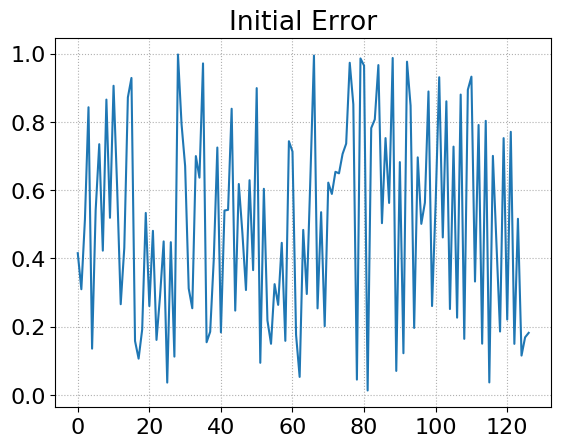
\includegraphics[width=0.45\textwidth]{../figures/gaussSeidelInitialErrRand}
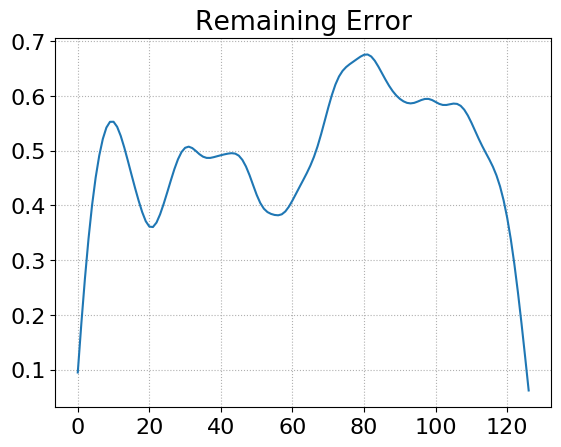
\includegraphics[width=0.45\textwidth]{../figures/gaussSeidelRemainingErrRand}
\end{center}
\end{frame}

% Slide
\begin{frame}{Basic iterative methods on a model problem}
\begin{block}{Behavior of Gauss-Seidel}
\bit
\item Smooth initial guess, no swift initial convergence...
\eit
\end{block}
\begin{center}
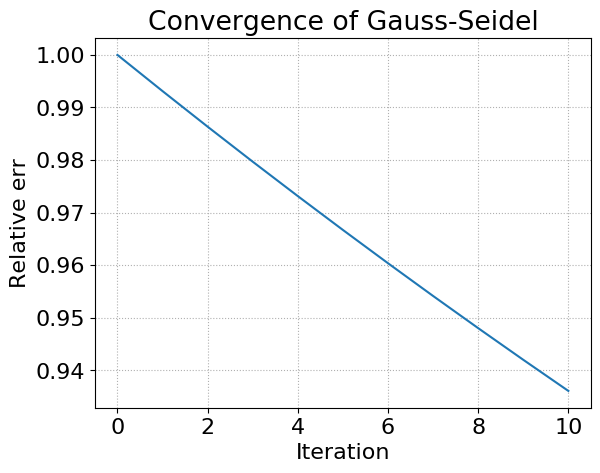
\includegraphics[width=0.5\textwidth]{../figures/gaussSeidelConvSmooth}
\end{center}
\end{frame}

% Slide
\begin{frame}{Basic iterative methods on a model problem}
\begin{block}{Behavior of Gauss-Seidel}
\bit
\item The starting smooth error is slow to change
\eit
\end{block}
\begin{center}
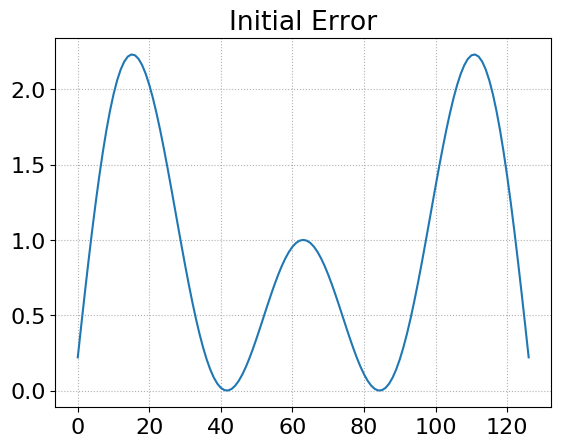
\includegraphics[width=0.45\textwidth]{../figures/gaussSeidelInitialErrSmooth}
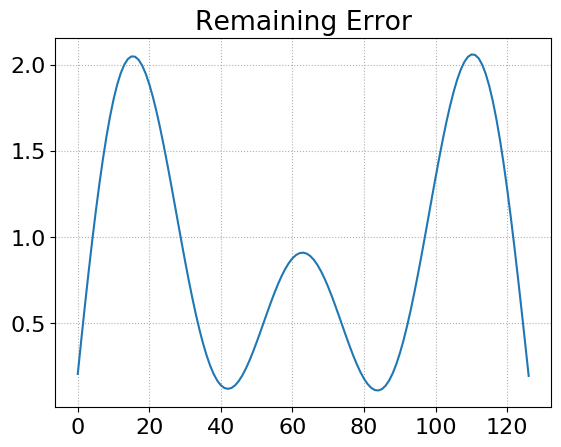
\includegraphics[width=0.45\textwidth]{../figures/gaussSeidelRemainingErrSmooth}
\end{center}
\end{frame}

% Slide
\begin{frame}{Basic iterative methods on a model problem}
\begin{block}{Behavior of Gauss-Seidel}
\bit
\item Observations:
\bit
\item Given a random initial guess, Gauss-Seidel reduces the error significantly on the first iteration
\item Convergence then stalls
\item Remaining error is smooth
\item Given a smooth initial guess, Gauss-Seidel is very slow
\eit
\item Seems that Gauss-Seidel is more effective at damping oscillatory error compared to smooth error
\eit
\end{block}
\end{frame}

% Slide
\begin{frame}{Basic iterative methods on a model problem}
\begin{block}{Review of eigenvalues and eigenvectors}
\bit
\item Eigenvalues, $\lambda_k$, and eigenvectors, $\mathbf{v}_k$, of a matrix, $A$, are defined by
\eq{
   A\mathbf{v}_k = \lambda_k \mathbf{v}_k
}
\item Evals and evecs can be a way to think about "action" of an operator: rotation and scaling
\item Important in many applications from physics and engineering
\eit
\end{block}
\end{frame}

% Slide
\begin{frame}{Basic iterative methods on a model problem}
\begin{block}{Review of eigenvalues and eigenvectors}
\bit
\item If $A$ is symmetric positive definite (SPD), then eigenvalues are real and positive and eigenvectors form an orthonormal basis for $\mathcal{R}^{N-1}$
\item Thus, any vector, $\mathbf{x}\in\mathcal{R}^{N-1}$ can be decomposed as 
\eq{
   \mathbf{x} = \sum_{k=1}^{N-1} \langle \mathbf{x}, \mathbf{v}_k \rangle \mathbf{v}_k 
}
\item We can study behavior of iterative methods by considering their effect on different eigenvectors
\eit
\end{block}
\end{frame}

% Slide
\begin{frame}{Basic iterative methods on a model problem}
\begin{block}{Evals and evecs of the model problem}
\bit
\item $A = tridiag(-1,2,-1)$, then the eigenvalues, $\lambda_k$, are
\eq{
   \lambda_k &= 4\sin^2\left(\frac{k\pi}{2N}\right), &k = 1,...,N-1 \\
}
\item The eigenvectors, $\mathbf{v}_k$, are defined componentwise as
\eq{
   v_{k,j} &= \sin\left(\frac{jk\pi}{N}\right), &j,k = 1,...,N-1 
}
\eit
\end{block}
\end{frame}

% Slide
\begin{frame}{Basic iterative methods on a model problem}
\begin{block}{Evals and evecs of the model problem}
\bit
\item Eigenvectors are the Fourier modes
\item Can study algorithm convergence by decomposing error into modes
\eit
\end{block}
\begin{center}
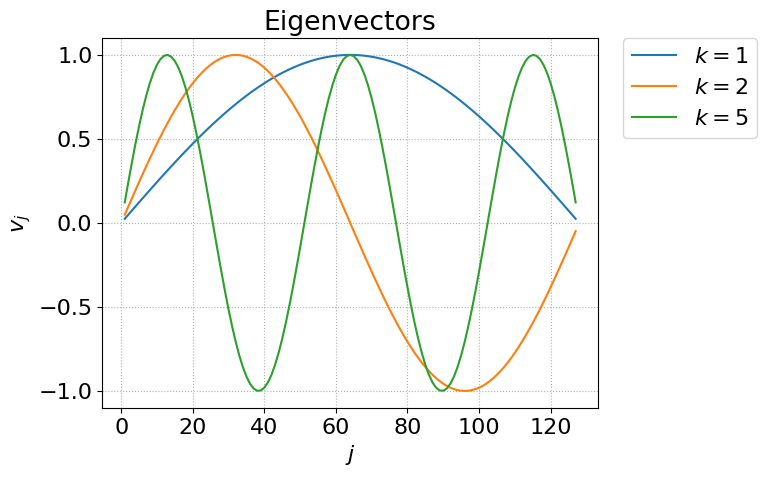
\includegraphics[width=0.6\textwidth]{../figures/eigenmodes}
\end{center}
\end{frame}

% Slide
\begin{frame}{Basic iterative methods on a model problem}
\begin{block}{Jacobi on the model problem}
\bit
\item Recall the Jacobi iteration
\eq{
   \mathbf{u} \leftarrow D^{-1}(\mathbf{f} + (L+U)\mathbf{u})
}
\item Jacobi is a matrix splitting iteration with error propagation matrix
\eq{
   E &= D^{-1}(L+U) \\
   &= I - D^{-1}A
}
\eit
\end{block}
\end{frame}

% Slide
\begin{frame}{Basic iterative methods on a model problem}
\begin{block}{Jacobi on the model problem}
\bit
\item $E$ and $A$ have the same evecs, $\mathbf{v}_k$
\eq{
   E\mathbf{v}_k &= (I - D^{-1}A)\mathbf{v}_k \\
   &= \mathbf{v}_k - D^{-1}(\lambda_k\mathbf{v}_k) & \text{(recall $D = 2I$)} \\
   &= (1 - \frac{1}{2}\lambda_k)\mathbf{v}_k
}
\item The evals, $\tilde\lambda_k$, of $E$ are related to those of $A$ 
\eq{
   \tilde\lambda_k &= 1 - \frac{1}{2}\lambda_k \\
   &= 1 - 2\sin^2\left(\frac{k\pi}{2N}\right)
}
\eit
\end{block}
\end{frame}


% Slide
\begin{frame}{Basic iterative methods on a model problem}
\begin{block}{Error reduction for Jacobi}
\bit
\item Given initial error, $\mathbf{e}^{(0)}$, error on the $i^th$ iteration is 
\eq{
   \mathbf{e}^{(i)} &= E^i\mathbf{e}^{(0)} \\
   &= E^i\left(\sum_{k=1}^{N-1} \langle \mathbf{e}^{(0)}, \mathbf{v}_k \rangle \mathbf{v}_k\right) \\
   &= \sum_{k=1}^{N-1} \tilde\lambda_k^i \langle \mathbf{e}^{(0)}, \mathbf{v}_k \rangle \mathbf{v}_k
}
\item So the $k^{th}$ "error mode" is reduced by $\tilde\lambda_k$ on each iteration
\eit
\end{block}
\end{frame}

% Slide
\begin{frame}{Basic iterative methods on a model problem}
\begin{block}{Error reduction for Jacobi}
\bit
\item Error modes associated with large and small evals are damped very slowly
\eq{
   \tilde\lambda_k = 1 - 2\sin^2\left(\frac{k\pi}{2N}\right)
}
\eit
\end{block}
\begin{center}
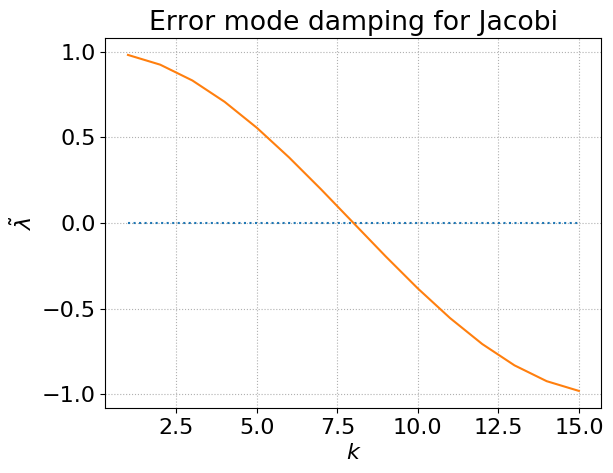
\includegraphics[width=0.5\textwidth]{../figures/jacobiModeDamping}
\end{center}
\end{frame}

% Slide
\begin{frame}{Basic iterative methods on a model problem}
\begin{block}{Error reduction for Jacobi}
\bit
\item For small $k$ (i.e. low "wave number"), Jacobi convergence is slow
\eit
\end{block}
\begin{center}
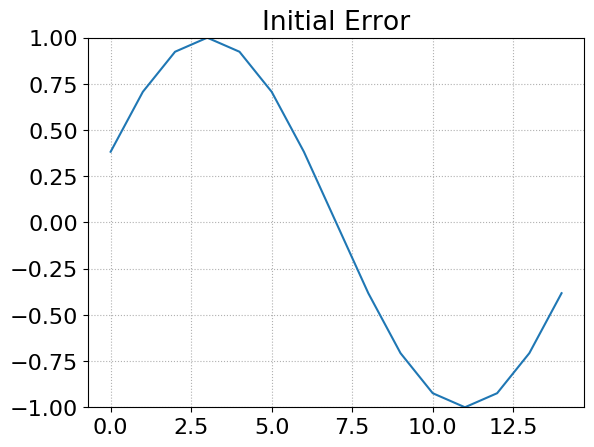
\includegraphics[width=0.45\textwidth]{../figures/jacobiInitialErrLowK}
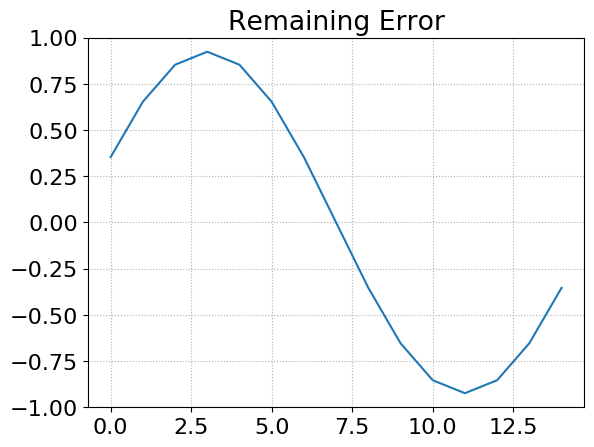
\includegraphics[width=0.45\textwidth]{../figures/jacobiRemainingErrLowK}
\end{center}
\end{frame}

% Slide
\begin{frame}{Basic iterative methods on a model problem}
\begin{block}{Error reduction for Jacobi}
\bit
\item Likewise for large $k$ (i.e. high wave number), Jacobi convergence is slow
\eit
\end{block}
\begin{center}
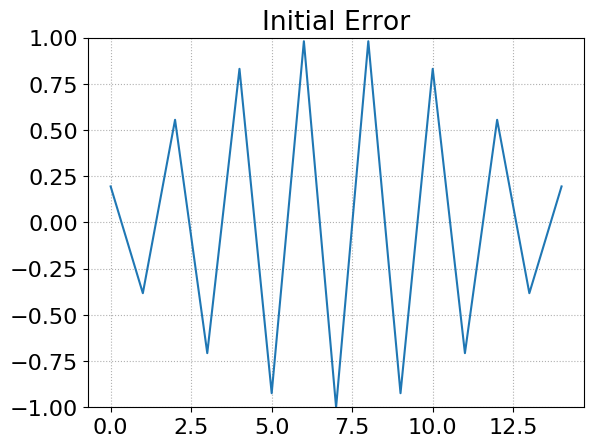
\includegraphics[width=0.45\textwidth]{../figures/jacobiInitialErrHighK}
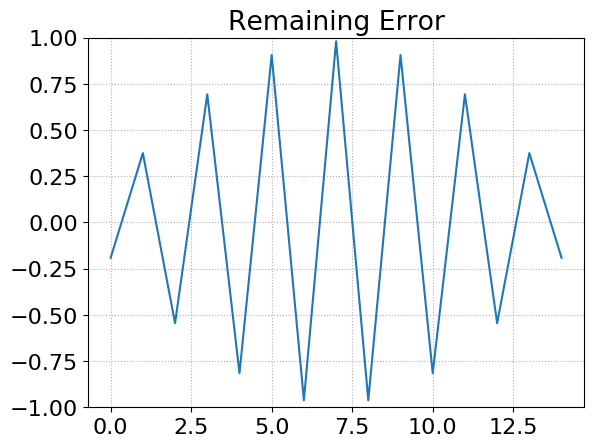
\includegraphics[width=0.45\textwidth]{../figures/jacobiRemainingErrHighK}
\end{center}
\end{frame}

% Slide
\begin{frame}{Basic iterative methods on a model problem}
\begin{block}{Error reduction for Jacobi}
\bit
\item Modes in the middle converge fast
\item If $N$ even, $k = N/2$, then $\tilde\lambda_k = 1 - 2\sin^2\left(\frac{k\pi}{2N}\right) = 0$
\eit
\end{block}
\begin{center}
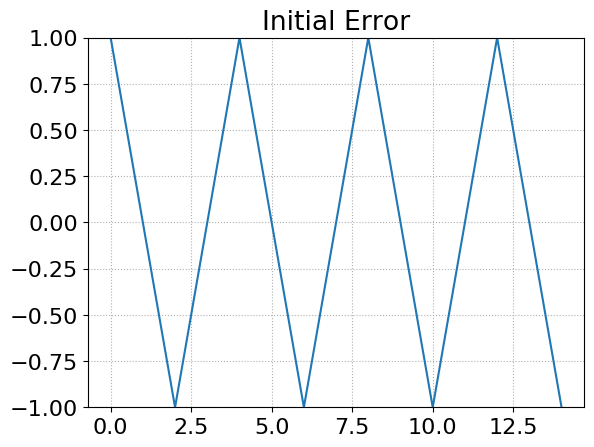
\includegraphics[width=0.45\textwidth]{../figures/jacobiInitialErrMiddleK}
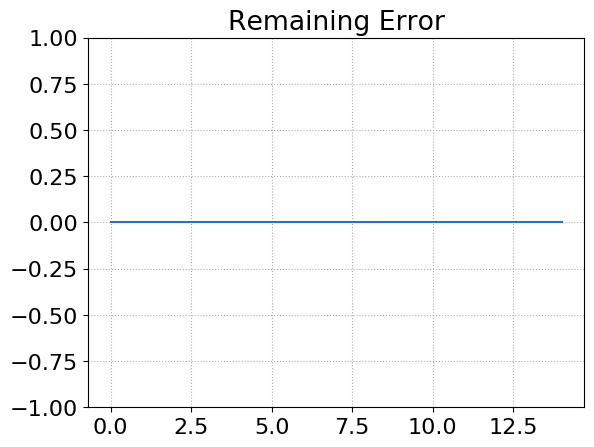
\includegraphics[width=0.45\textwidth]{../figures/jacobiRemainingErrMiddleK}
\end{center}
\end{frame}

% Slide
\begin{frame}{Basic iterative methods on a model problem}
\begin{block}{Weighted Jacobi}
\bit
\item In practice, Jacobi is usually modified with a weighting parameter, $\omega$
\eq{
   \mathbf{u} \leftarrow (1 - \omega)\mathbf{u} + \omega D^{-1}(\mathbf{f} + (L+U)\mathbf{u})
}
\item The error propagation matrix in this case is
\eq{
   E &= I - \omega D^{-1}A
}
\item The associated evals are
\eq{
   \tilde\lambda_k &= 1 - 2\omega\sin^2\left(\frac{k\pi}{2N}\right)
}
\eit
\end{block}
\end{frame}

% Slide
\begin{frame}{Basic iterative methods on a model problem}
\begin{center}
\begin{block}{Error reduction for Jacobi}
\bit
\item With appropriate $\omega$, can effectively damp modes associated with large $k$
\eq{
   \tilde\lambda_k = 1 - 2\omega\sin^2\left(\frac{k\pi}{2N}\right)
}
\eit
\end{block}
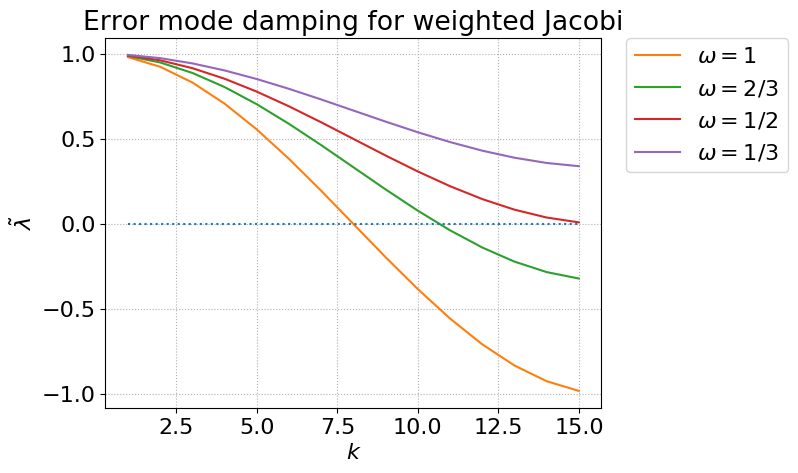
\includegraphics[width=0.6\textwidth]{../figures/weightedJacobiModeDamping}
\end{center}
\end{frame}

% Slide
\begin{frame}{Basic iterative methods on a model problem}
\begin{block}{Gauss-Seidel}
\bit
\item Gauss-Seidel exibits similar behavior
\item Evecs of error propagation, $E$, for Gauss-Seidel are not the same as the evecs of $A$
\item Gauss-Seidel also damps the evecs of $A$ associated with large evals
\eit
\end{block}
\end{frame}

%%%%%%%%%%%%%%%%%%%%%%%%%%%%%%%%%%%%%%%%%%%%%%%%%%%%%%%%%%%%%%%%%%%%%%%%%%%%%%%%

\section{Towards multigrid}

% Slide
\begin{frame}{Towards multigrid}
\begin{block}{Observations}
\bit
\item Weighted Jacobi and Gauss-Seidel are not good solvers on their own
\item They do a good job at damping certain error modes for the model problem
\item Specifically, they remove "high-frequency" error (they damp the oscillatory evecs of $A$)
\item Call these "smoothers" or "relaxation methods"
\eit
\end{block}
\end{frame}

% Slide
\begin{frame}{Towards multigrid}
\begin{block}{Observations}
\bit
\item Smooth modes are representable on a coarser grid
\item Furthermore, they are relatively more oscillatory on that grid 
\eit
\end{block}
\only<1>{
\begin{center}
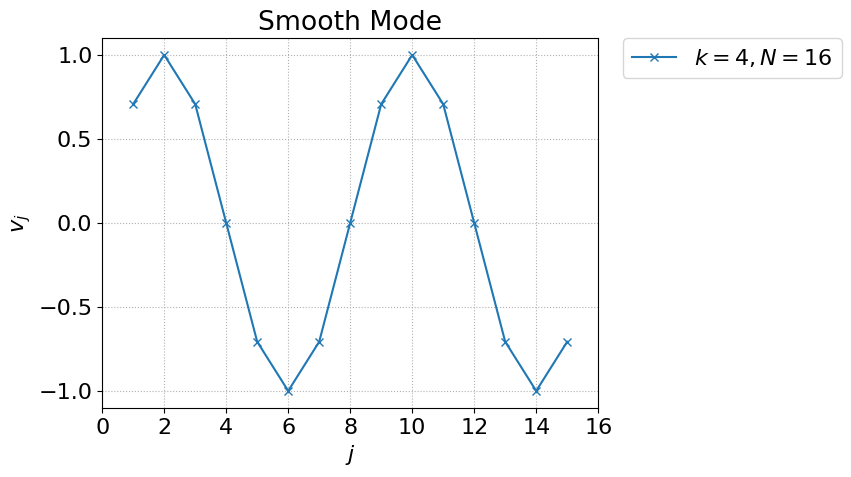
\includegraphics[width=0.6\textwidth]{../figures/smoothMode}
\end{center}
}
\only<2>{
\begin{center}
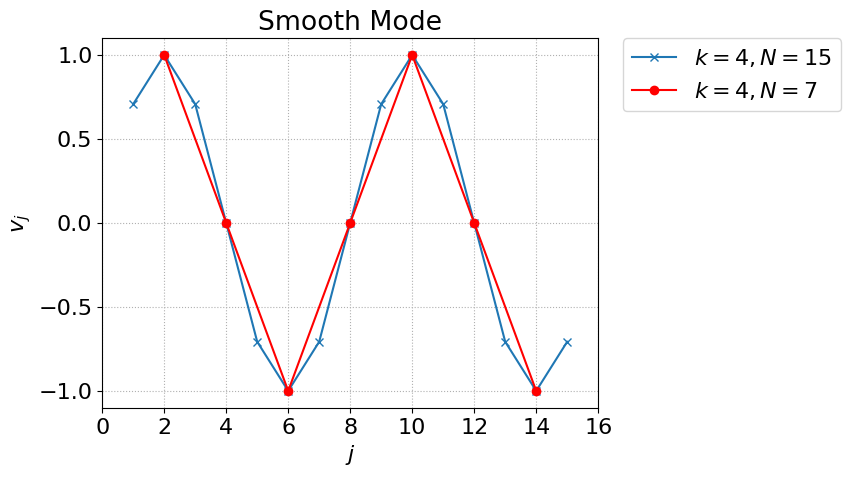
\includegraphics[width=0.6\textwidth]{../figures/modeCoarse}
\end{center}
}
\end{frame}

% Slide
\begin{frame}{Towards multigrid}
\begin{block}{Observations}
\bit
\item Recall that relaxation makes the error, $\mathbf{e}$, smooth (even if the solution, $\mathbf{u}$, is oscillatory)
\item The error satisfies the residual equation
\eq{
   A\mathbf{e} = \mathbf{r}
}
\item Solve on a coarse grid to obtain an approximation to error after relaxation
\eit
\end{block}
\end{frame}

% Slide
\begin{frame}{Towards multigrid}
\begin{block}{Coarse-grid correction}
\bit
\item After some Gauss-Seidel iterations, convergence stalls...
\eit
\end{block}
\begin{center}
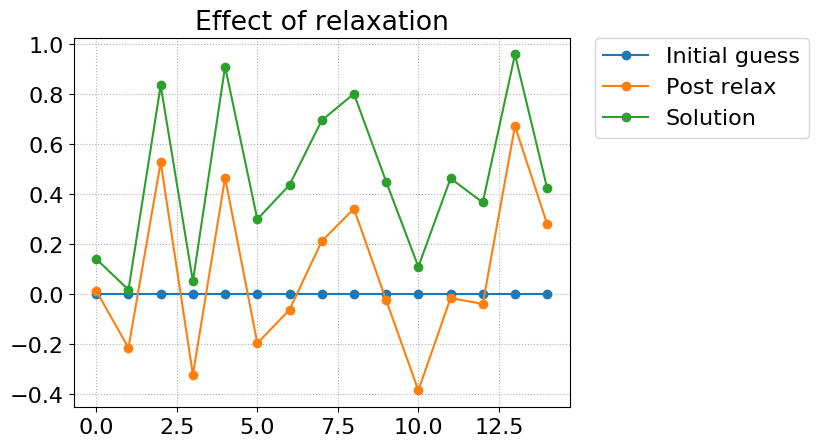
\includegraphics[width=0.7\textwidth]{../figures/solnPostRelax}
\end{center}
\end{frame}

% Slide
\begin{frame}{Towards multigrid}
\begin{block}{Coarse-grid correction}
\bit
\item ... but the error is smooth
\eit
\end{block}
\begin{center}
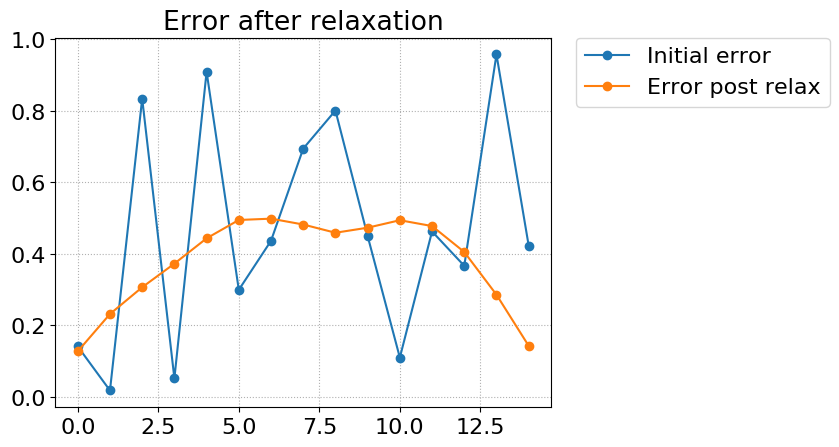
\includegraphics[width=0.7\textwidth]{../figures/errPostRelax}
\end{center}
\end{frame}

% Slide
\begin{frame}{Towards multigrid}
\begin{block}{Coarse-grid correction}
\bit
\item Solving for the error on a coarse-grid yields a good approximation
\eit
\end{block}
\begin{center}
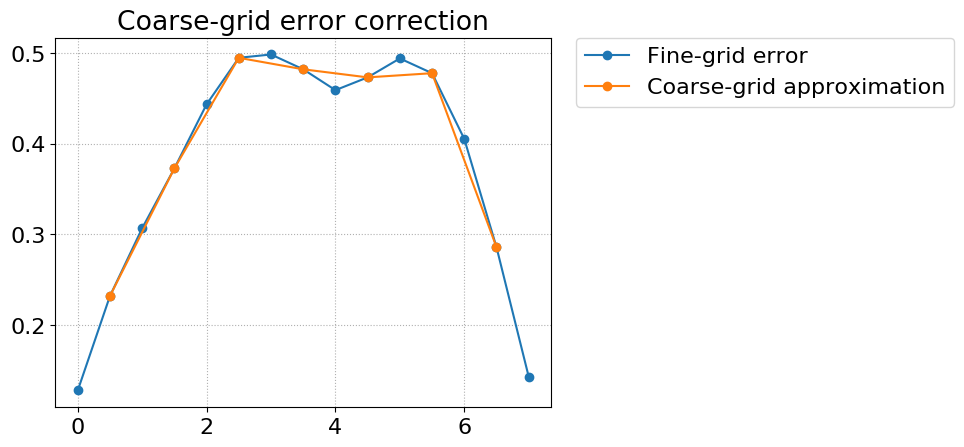
\includegraphics[width=0.7\textwidth]{../figures/coarseGridErr}
\end{center}
\end{frame}

% Slide
\begin{frame}{Towards multigrid}
\begin{block}{Coarse-grid correction}
\bit
\item Adding the coarse-grid correction yields a much better fine-grid solution
\eit
\end{block}
\begin{center}
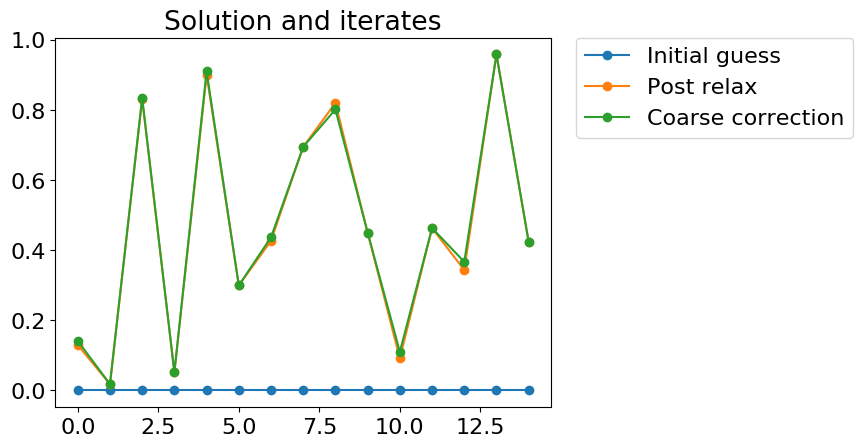
\includegraphics[width=0.7\textwidth]{../figures/solnCoarseCorrect}
\end{center}
\end{frame}

% Slide
\begin{frame}{Towards multigrid}
\begin{block}{Coarse-grid correction}
\bit
\item Relax on $A^f\mathbf{u}^f = \mathbf{f}^f$ to obtain approximate fine-grid solution
\item Error, $\mathbf{e}^f = \mathbf{\tilde u} - \mathbf{u}^f$, is smooth
\item Calculate the residual $\mathbf{r}^f = \mathbf{f}^f - A^f\mathbf{u}^f$
\item Solve $A^c\mathbf{e}^c = \mathbf{r}^c$ to obtain a coarse-grid correction
\item Correct on the fine grid $\mathbf{u}^f \leftarrow \mathbf{u}^f + \mathbf{e}^f$
\eit
\end{block}
\end{frame}

% Slide
\begin{frame}{Towards multigrid}
\begin{block}{Coarse-grid correction}
\bit
\item The coarse-grid system, $A^c\mathbf{e}^c = \mathbf{r}^c$, is smaller
\item Recall that smooth modes look more oscillatory there
\item Relaxation is effective again!
\item To solve for even smoother error modes, can go to further coarse grids
\eit
\end{block}
\end{frame}

% Slide
\begin{frame}{Towards multigrid}
\begin{block}{Remaining questions}
\bit
\item How to define the coarse grid?
\item How to move between grid levels?
\item How to go from two-grid to multigrid?
\eit
\end{block}
\end{frame}

%%%%%%%%%%%%%%%%%%%%%%%%%%%%%%%%%%%%%%%%%%%%%%%%%%%%%%%%%%%%%%%%%%%%%%%%%%%%%%%%

\section{Components of multigrid}

% Slide
\begin{frame}{Components of multigrid}
\begin{block}{Components of multigrid}
\bit
\item Hierarchy of grids and associated problems
\item Relaxation methods to apply to problems on each grid level
\item Interpolation from coarse to fine grids
\item Restriction from fine to coarse grids
\item Cycle structure
\eit
\end{block}
\end{frame}

% Slide
\begin{frame}{Components of multigrid}
\begin{block}{Coarse grids}
\bit
\item Rediscretize the PDE with half the step size
\eit
\end{block}
\begin{center}
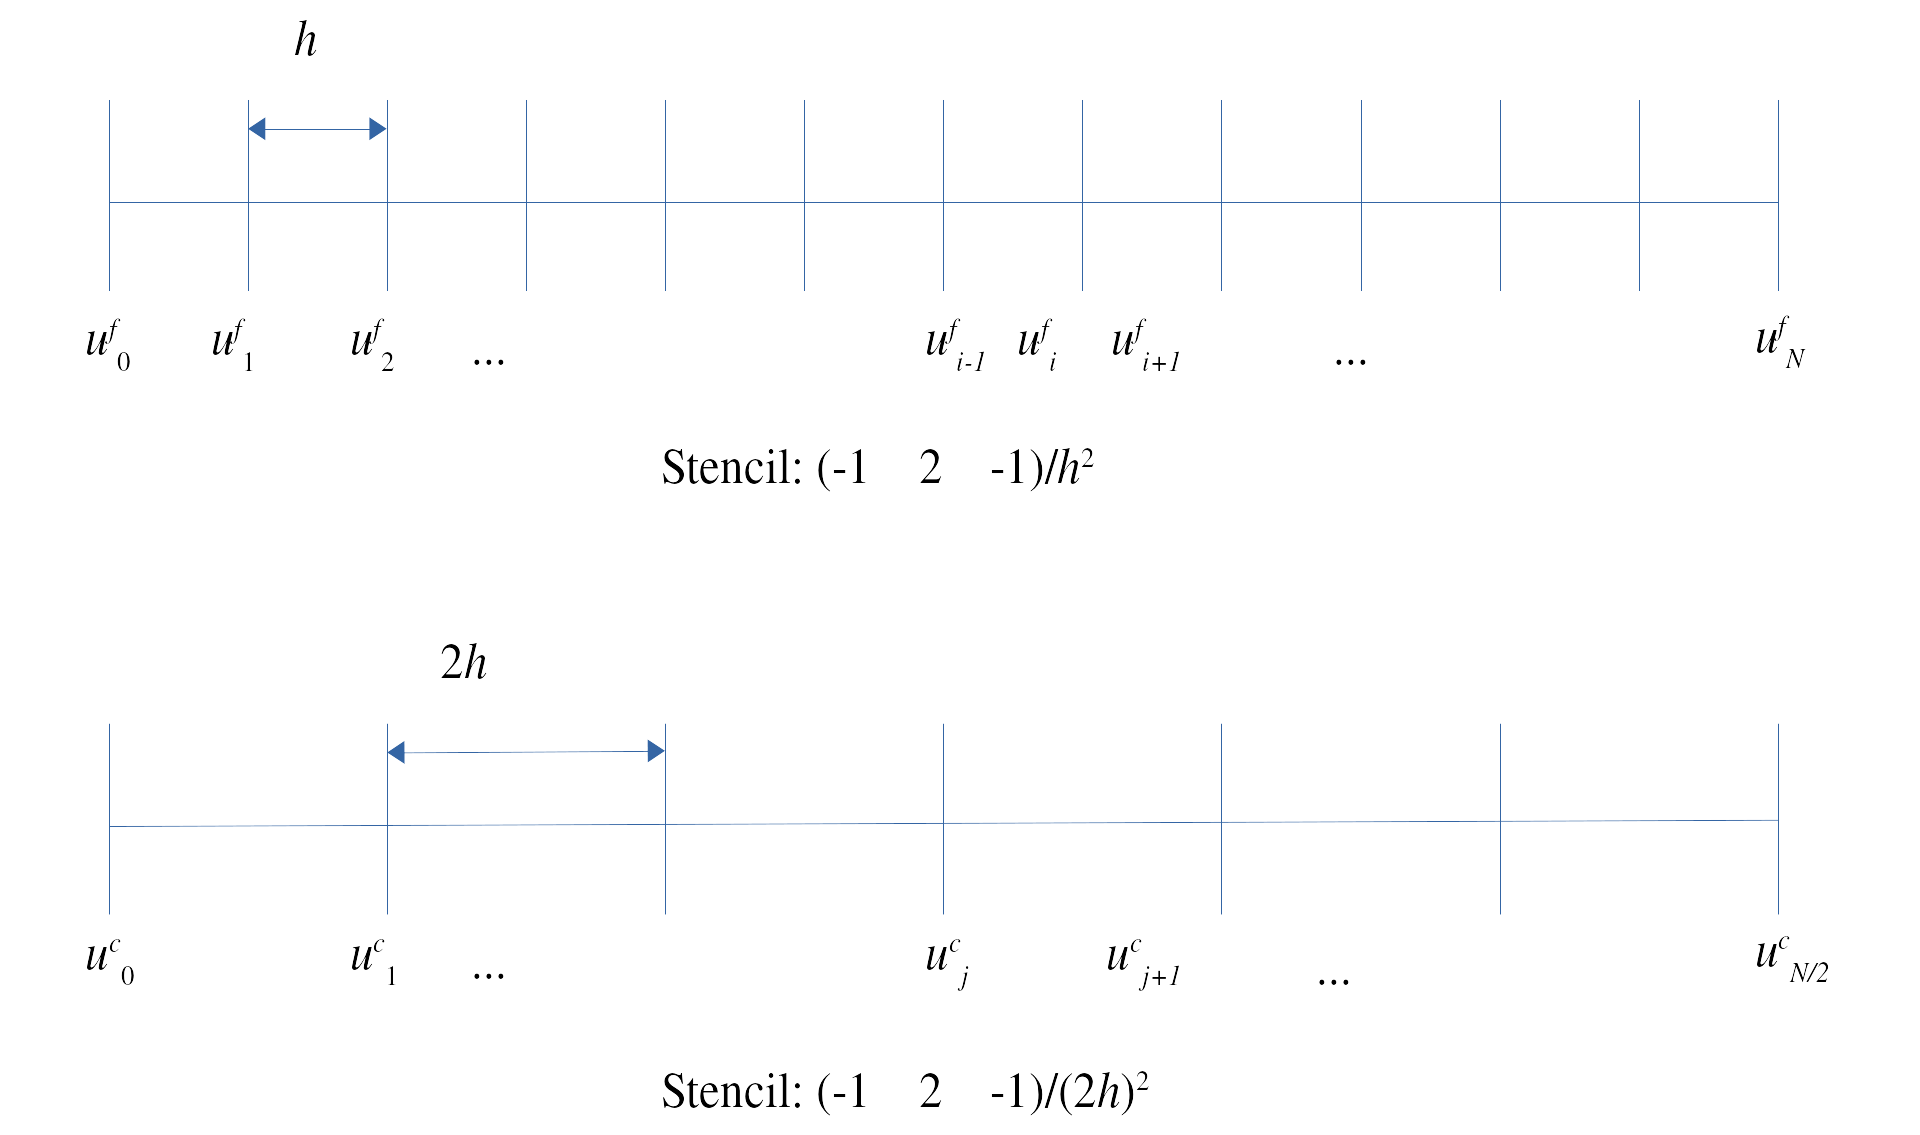
\includegraphics[width=0.7\textwidth]{../figures/coarse1DFDPoisson}
\end{center}
\end{frame}

% Slide
\begin{frame}{Components of multigrid}
\begin{block}{Interpolation (prolongation)}
\bit
\item Linear interpolation
\item Identity at C-points
\item Average of neighbors at F-points
\eq{
   e^f_i = \begin{cases}
   e^c_{i/2}, &i \,\,\text{even} \\
   \frac{1}{2}(e^c_{(i-1)/2} + e^c_{(i+1)/2}), &i \,\,\text{odd}
   \end{cases}
}
\eit
\end{block}
\end{frame}

% Slide
\begin{frame}{Components of multigrid}
\begin{block}{Interpolation (prolongation)}
\bit
\item Linear interpolation accurately reproduces smooth fine-grid error from a coarse representation
\eit
\end{block}
\only<1>{
\begin{center}
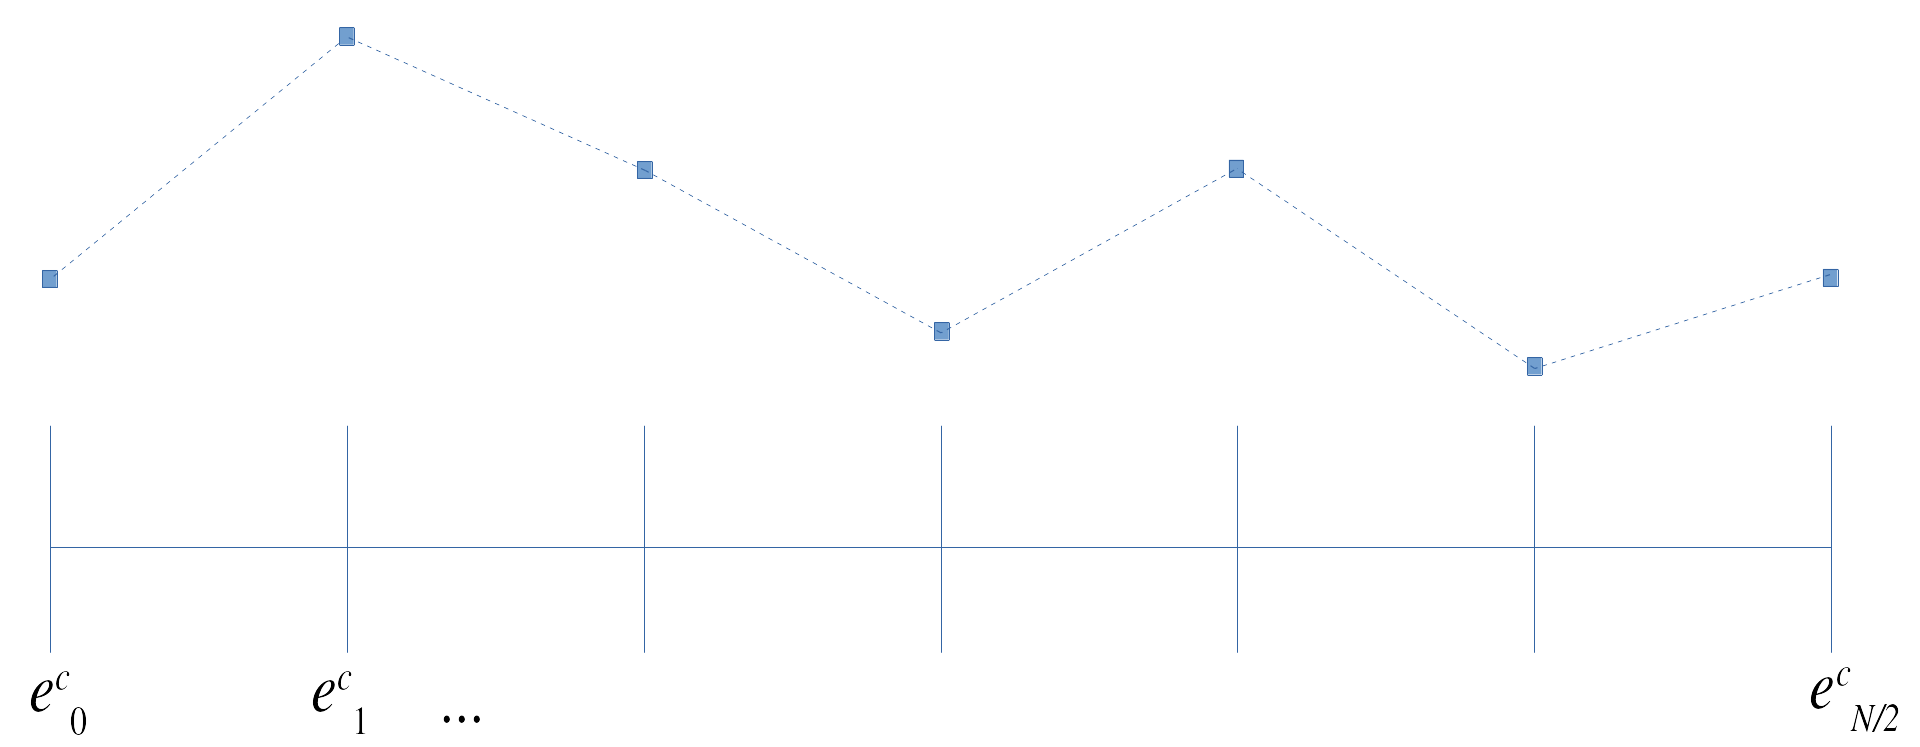
\includegraphics[width=0.7\textwidth]{../figures/coarseError}
\end{center}
}
\only<2>{
\begin{center}
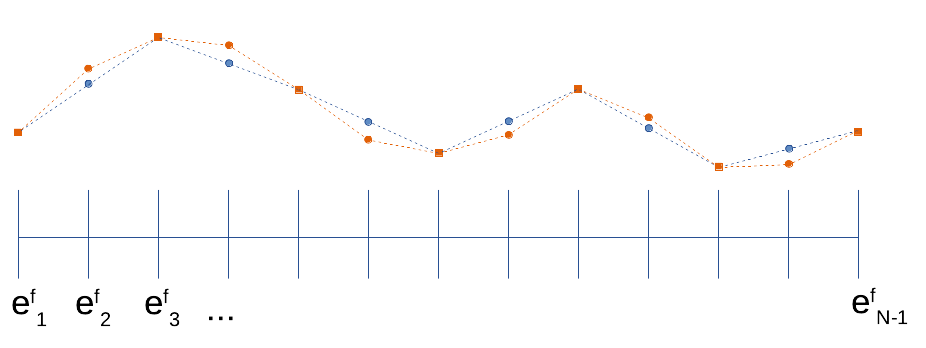
\includegraphics[width=0.7\textwidth]{../figures/coarseCorrectionSmooth}
\end{center}
}
\end{frame}

% Slide
\begin{frame}{Components of multigrid}
\begin{block}{Interpolation (prolongation)}
\bit
\item If the fine-grid error is oscillatory, linear interpolation from the coarse grid is not so accurate
\eit
\end{block}
\begin{center}
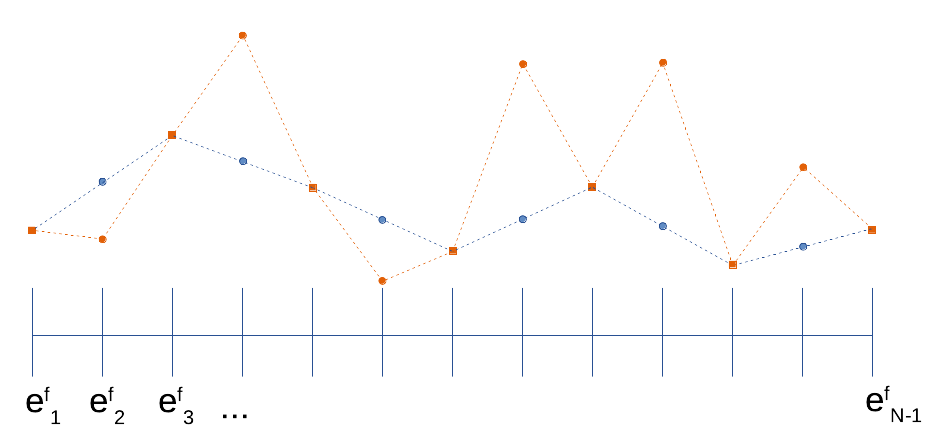
\includegraphics[width=0.7\textwidth]{../figures/coarseCorrectionOscillatory}
\end{center}
\end{frame}

% Slide
\begin{frame}{Components of multigrid}
\begin{block}{Interpolation (prolongation)}
\bit
\item Matrix form of interpolation, $P\in\mathcal{R}^{(N-1)\times(N/2-1)}$
\eit
\eq{
   \begin{bmatrix}
   1/2 & & & \\
   1 & & & \\
   1/2 & 1/2 & & \\
    & 1 & \ddots & \\
    & \ddots & & \\
    &  & 1/2 & 1/2 \\
    &  & & 1 \\
    &  & & 1/2 \\
   \end{bmatrix}
   \begin{bmatrix}
   e^c_1 \\
   e^c_2 \\
   \vdots \\
   e^c_{N/2-1}
   \end{bmatrix}
   =
   \begin{bmatrix}
   e^f_1 \\
   e^f_2 \\
   \\
   \vdots \\
   \\
   e^f_{N-1}
   \end{bmatrix}
}
\end{block}
\end{frame}

% Slide
\begin{frame}{Components of multigrid}
\begin{block}{Restriction}
\bit
\item Restriction by injection: C-points retain their value, F-points do not contribute
\eit
\eq{
   r^c_i = r^f_{2i}
}
\end{block}
\end{frame}

% Slide
\begin{frame}{Components of multigrid}
\begin{block}{Restriction}
\bit
\item Restriction by injection: C-points retain their value, F-points do not contribute
\eit
\end{block}
\only<1>{
\begin{center}
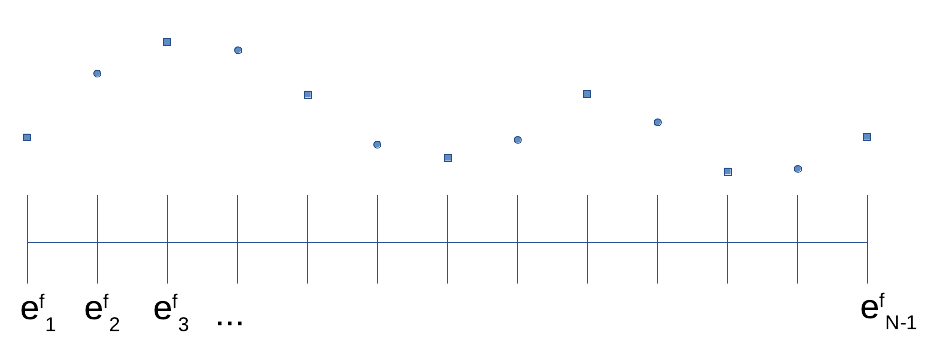
\includegraphics[width=0.7\textwidth]{../figures/fineResidual}
\end{center}
}
\only<2>{
\begin{center}
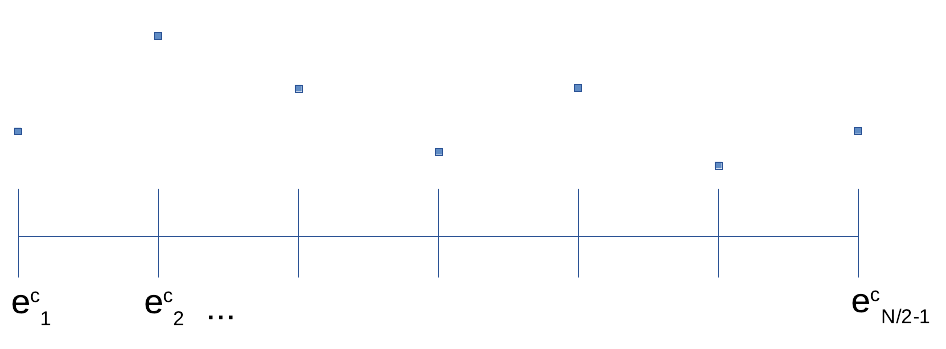
\includegraphics[width=0.7\textwidth]{../figures/injectedResidual}
\end{center}
}
\end{frame}

% Slide
\begin{frame}{Components of multigrid}
\begin{block}{Restriction}
\bit
\item Matrix form of injection restriction, $R\in\mathcal{R}^{(N/2-1)\times(N-1)}$
\eit
\eq{
   \begin{bmatrix}
    0 & 1 & 0& & & & \\
    & & 0 & 1 & 0 & & \\
    & & & \ddots & \ddots & & \\
    & & & & & & \\
    & & & & 0 & 1 & 0\\
   \end{bmatrix}
   \begin{bmatrix}
   r^f_1 \\
   r^f_2 \\
   \\
   \vdots \\
   \\
   r^f_{N-1}
   \end{bmatrix}
   =
   \begin{bmatrix}
   r^c_1 \\
   r^c_2 \\
   \vdots \\
   r^c_{N/2-1}
   \end{bmatrix}
}
\end{block}
\end{frame}

% Slide
\begin{frame}{Components of multigrid}
\begin{block}{Restriction}
\bit
\item Restriction by full-weighting: weighted average of C-points with their neighboring F-points
\eit
\eq{
   r^c_i = \frac{1}{4}r^f_{2i-1} + \frac{1}{2}r^f_{2i} + \frac{1}{4}r^f_{2i+1}
}
\end{block}
\end{frame}

% Slide
\begin{frame}{Components of multigrid}
\begin{block}{Restriction}
\bit
\item Restriction by full-weighting: weighted average of C-points with their neighboring F-points
\eit
\end{block}
\begin{center}
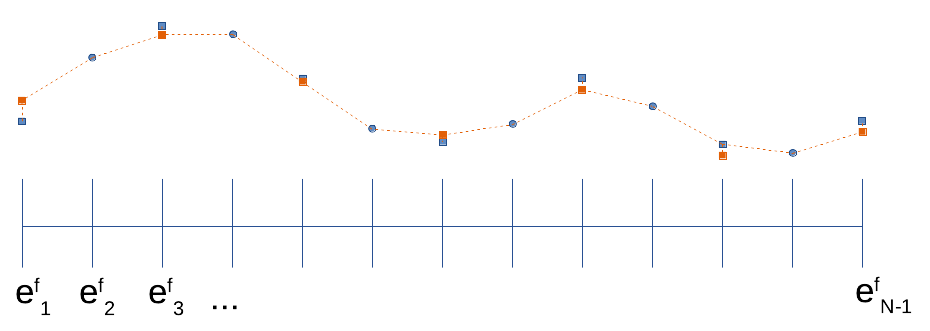
\includegraphics[width=0.7\textwidth]{../figures/fullWeightingResidual}
\end{center}
\end{frame}


% Slide
\begin{frame}{Components of multigrid}
\begin{block}{Restriction}
\bit
\item Matrix form of full-weighting restriction, $R\in\mathcal{R}^{(N/2-1)\times(N-1)}$
\eit
\eq{
   \begin{bmatrix}
    1/4 & 1/2 & 1/4 & & & & \\
    & & 1/4 & 1/2 & 1/4 & & \\
    & & & \ddots & \ddots & & \\
    & & & & & & \\
    & & & & 1/4 & 1/2 & 1/4 \\
   \end{bmatrix}
   \begin{bmatrix}
   r^f_1 \\
   r^f_2 \\
   \\
   \vdots \\
   \\
   r^f_{N-1}
   \end{bmatrix}
   =
   \begin{bmatrix}
   r^c_1 \\
   r^c_2 \\
   \vdots \\
   r^c_{N/2-1}
   \end{bmatrix}
}
\end{block}
\end{frame}

% Slide
\begin{frame}{Components of multigrid}
\begin{block}{Full-weighting and the Galerkin coarse-grid operator}
\bit
\item Note that with full-weighting, $R = sP^T$, with $s = 1/2$
\item This relationship between interpolation and restriction is enforced in many multigrid hierarchies and yields nice properties
\item For the model problem, if $R = sP^T$, then rediscretization on the coarse grid is equivalent to $A^c = RA^fP$
\item $A^c = RA^fP$ is the Galerkin coarse-grid operator
\item Note that if $A$ is symmetric and $R = sP^T$, then $A^c$ is symmetric
\eit
\end{block}
\end{frame}

% Slide
\begin{frame}{Components of multigrid}
\begin{block}{Two-grid cycle}
\begin{algorithm}[H]
\caption{Two-grid cycle}
\begin{algorithmic}
\State Set $\mathbf{u}$ initial guess
\State Relax on $A^f\mathbf{u}^f = \mathbf{f}^f$
\State Calculate residual $\mathbf{r}^f = \mathbf{f}^f - A^f\mathbf{u}^f$
\State Restrict residual $\mathbf{r}^c = R\mathbf{r}^f$
\State Solve on the coarse grid $A^c\mathbf{e}^c = \mathbf{r}^c$
\State Interpolate coarse-grid correction $\mathbf{u}^f = \mathbf{u}^f + P\mathbf{e}^c$
\State Relax again on $A^f\mathbf{u}^f = \mathbf{f}^f$
\end{algorithmic}
\end{algorithm}
\end{block}
\end{frame}

%%%%%%%%%%%%%%%%%%%%%%%%%%%%%%%%%%%%%%%%%%%%%%%%%%%%%%%%%%%%%%%%%%%%%%%%%%%%%%%%

\section{Multigrid cycles}

% Slide
\begin{frame}{Multigrid cycles}
\begin{block}{From two level to multilevel}
\bit
\item The simplest way to go from the two-grid cycle to a multigrid cycle is to recurse
\item Instead of an exact solve on the coarse grid, solve via relaxation and further coarse-grid correction
\item Result is a multigrid V-cycle
\eit
\end{block}
\end{frame}

% Slide
\begin{frame}{Multigrid cycles}

\begin{algorithm}[H]
\caption{Recursive V-cycle$(\mathbf{u},\mathbf{f})$}
\begin{algorithmic}
\State Relax on $A\mathbf{u} = \mathbf{f}$
\State Calculate residual $\mathbf{r} = \mathbf{f} - A\mathbf{u}$
\State Restrict residual $\mathbf{r}^c = R\mathbf{r}$

\If{Coarse-grid system, $A^c$, is small enough for direct solve}
\State $\mathbf{e}^c = (A^c)^{-1}\mathbf{r}^c$
\Else
\State Set $\mathbf{e}^c = \mathbf{0}$
\State Call recursive V-cycle$(\mathbf{e}^c, \mathbf{r}^c)$
\EndIf
\State Interpolate coarse-grid correction $\mathbf{u} = \mathbf{u} + P\mathbf{e}^c$
\State Relax again on $A\mathbf{u} = \mathbf{f}$
\end{algorithmic}
\end{algorithm}
\end{frame}

% Slide
\begin{frame}{Multigrid cycles}
\begin{center}
\hspace{-1cm}
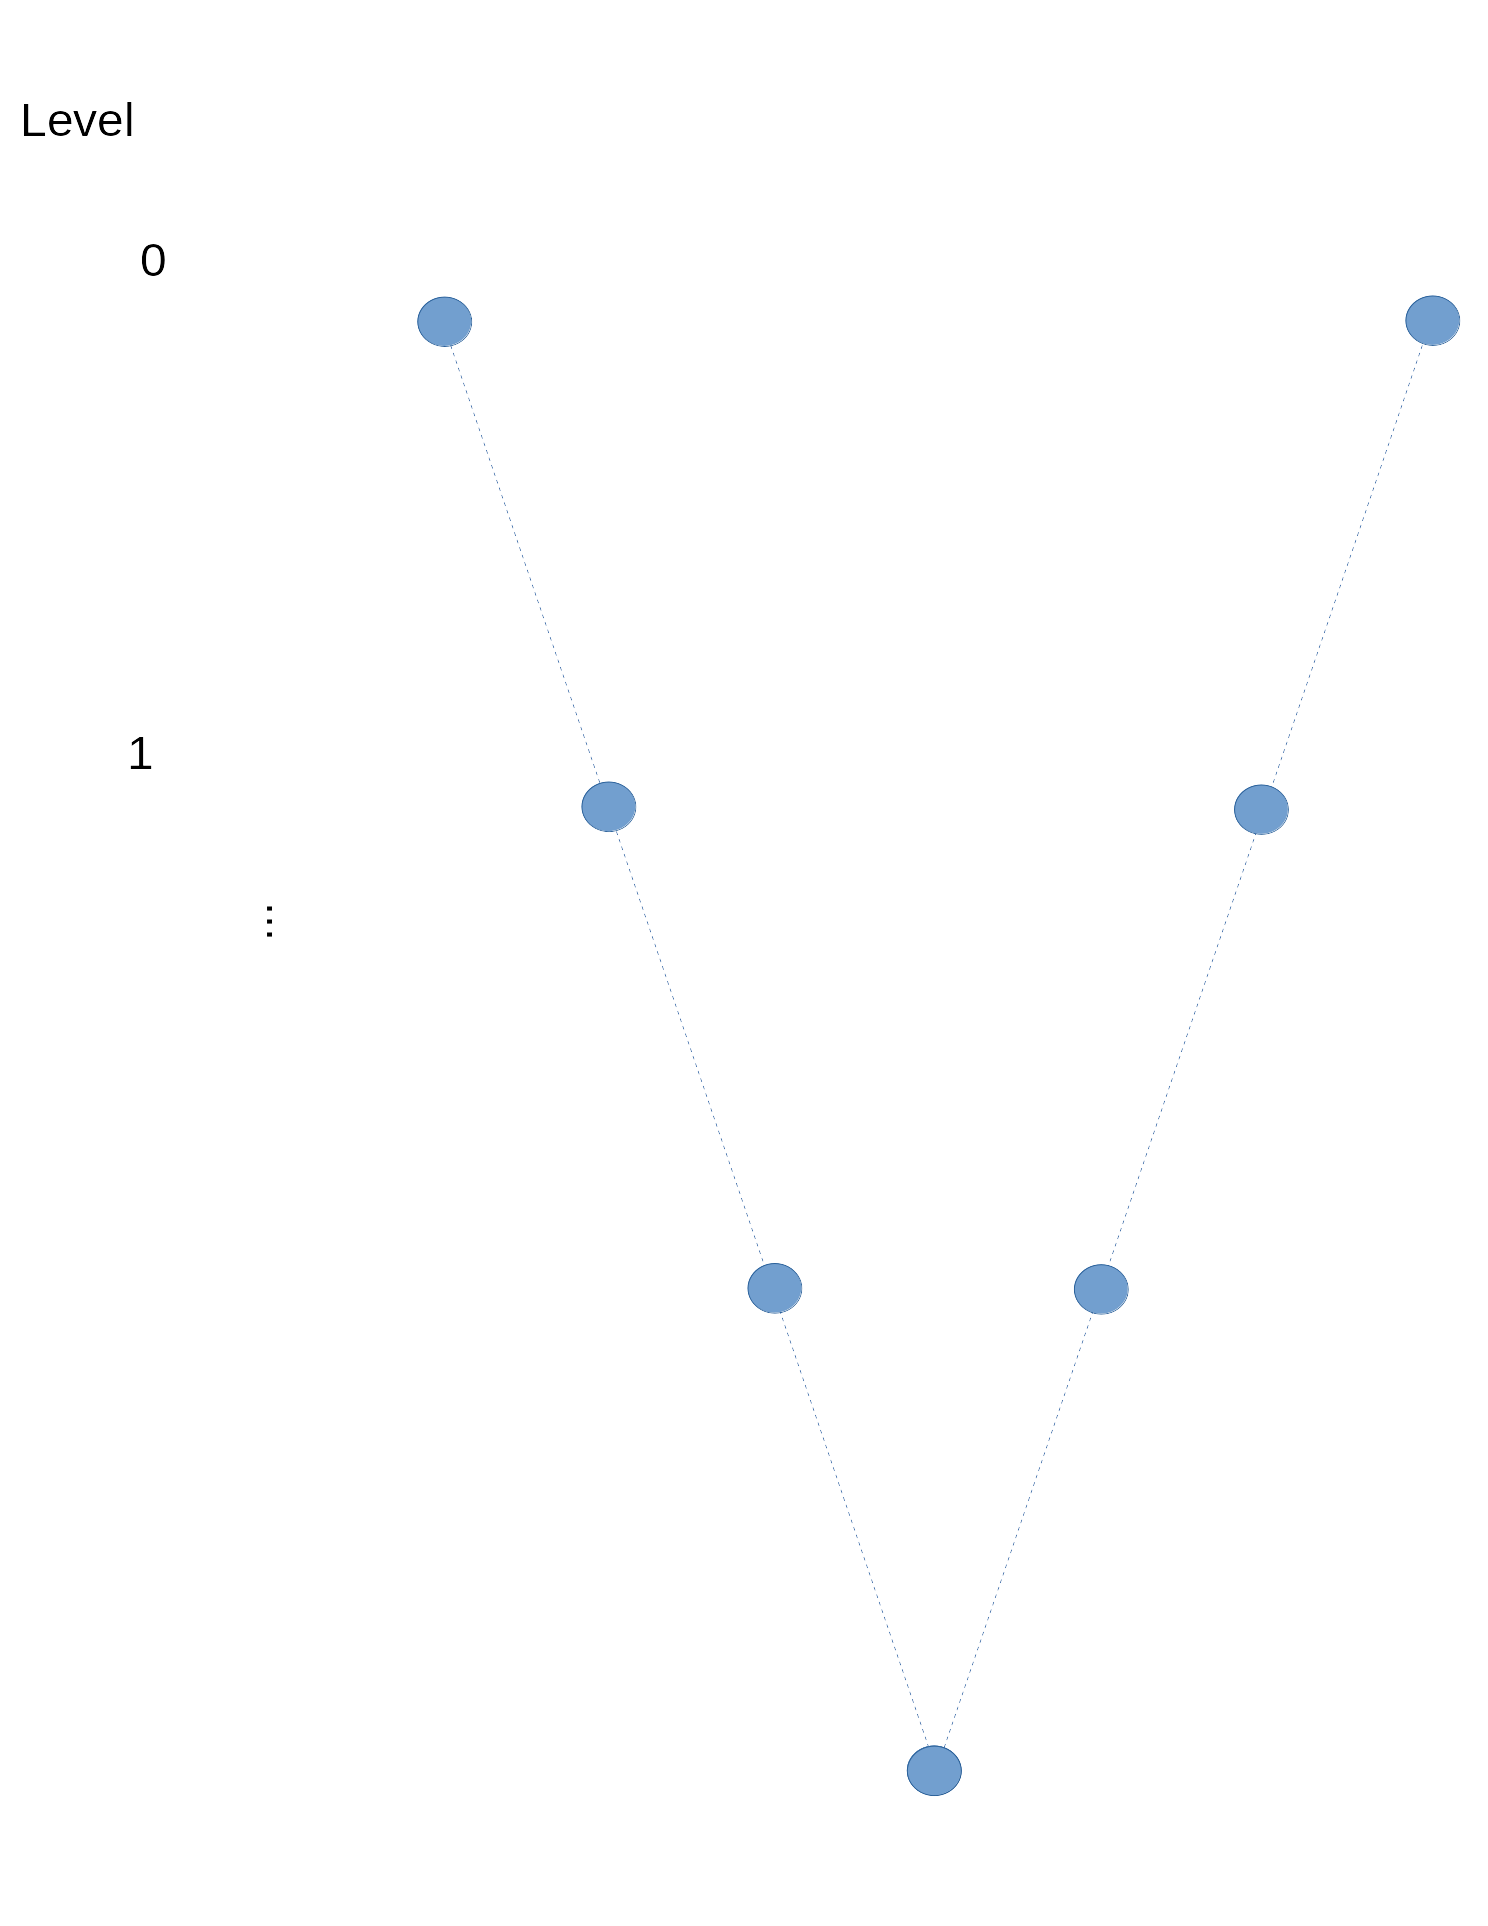
\includegraphics[width=0.5\textwidth]{../figures/Vcycle}
\end{center}
\end{frame}

% Slide
\begin{frame}{Multigrid cycles}
\begin{block}{V-cycle cost}
\bit
\item Recall the claim that multigrid has optimal, $O(N)$ computational cost
\item Define a "work unit" (WU) as the cost of one mat-vec on the fine grid, $A\mathbf{u}$
\item If $A$ is sparse, then one WU has $O(N)$ cost
\item Point-wise relaxation (e.g. Gauss-Seidel) costs one WU
\eit
\end{block}
\end{frame}

% Slide
\begin{frame}{Multigrid cycles}
\begin{block}{V-cycle cost}
\bit
\item Assume regular, $d$-dimensional grids and a constance coarsening factor, $C$
\item Then the total number of WU for two relaxations and a residual calculation on level $l$ is $\approx 3/C^{ld}$
\item Summing over the levels yields the cost for a V-cycle
\eq{
  \text{Total cost in WU } \approx \sum_{l=0}^{L-1} \frac{3}{C^{ld}} \leq \frac{3}{1 - C^{-d}}
}
\item For 1D model problem, total cost is less than 6 WU.
\eit
\end{block}
\end{frame}


% Slide
\begin{frame}{Multigrid cycles}
\begin{block}{Other cycle types}
\bit
\item V-cycles are very common in practice
\item More generally, V$(\nu_1, \nu_2)$-cycles perform $\nu_1$ pre-relaxations and $\nu_2$ post-relaxations
\item Can also use different cycle structures (visit the grid levels in different orders)
\eit
\end{block}
\end{frame}

% Slide
\begin{frame}{Multigrid cycles}
\begin{algorithm}[H]
\caption{Recursive W-cycle$(\mathbf{u},\mathbf{f})$}
\begin{algorithmic}
\State Relax on $A\mathbf{u} = \mathbf{f}$
\State Calculate residual $\mathbf{r} = \mathbf{f} - A\mathbf{u}$
\State Restrict residual $\mathbf{r}^c = R\mathbf{r}$

\If{Coarse-grid system, $A^c$, is small enough for direct solve}
\State $\mathbf{e}^c = (A^c)^{-1}\mathbf{r}^c$
\Else
\State Set $\mathbf{e}^c = \mathbf{0}$
\State Call recursive W-cycle$(\mathbf{e}^c, \mathbf{r}^c)$
\State Call recursive W-cycle$(\mathbf{e}^c, \mathbf{r}^c)$ again
\EndIf
\State Interpolate coarse-grid correction $\mathbf{u} = \mathbf{u} + P\mathbf{e}^c$
\State Relax again on $A\mathbf{u} = \mathbf{f}$
\end{algorithmic}
\end{algorithm}
\end{frame}

% Slide
\begin{frame}{Multigrid cycles}
\begin{center}
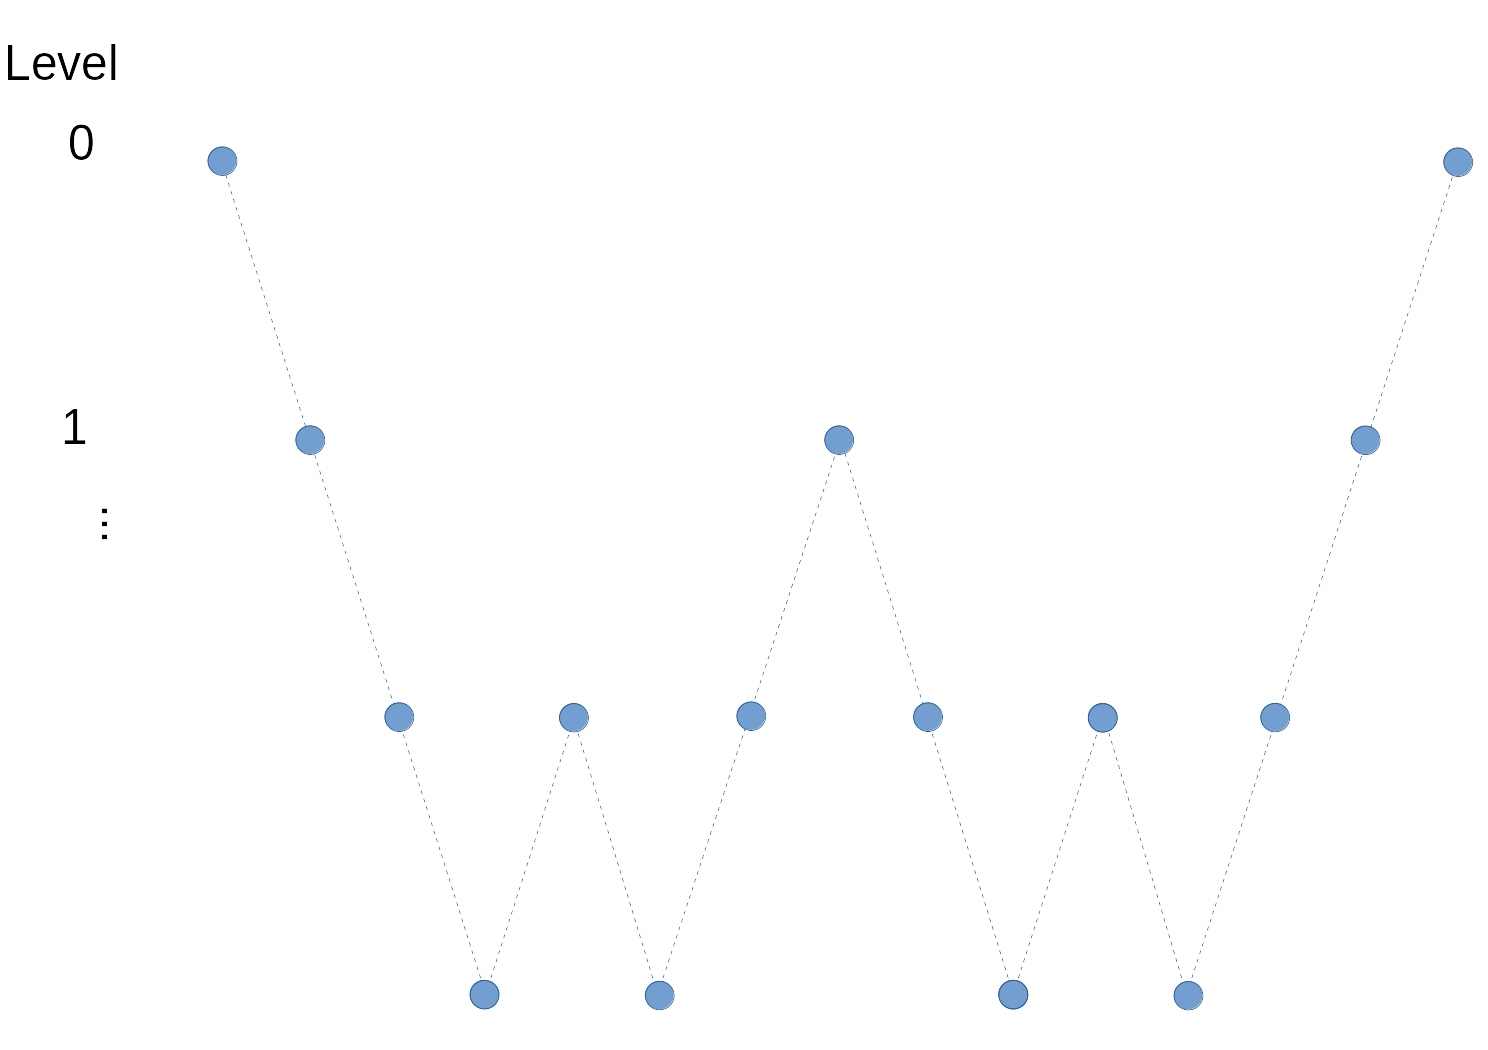
\includegraphics[width=0.7\textwidth]{../figures/Wcycle}
\end{center}
\end{frame}

% Slide
\begin{frame}{Multigrid cycles}
\begin{block}{Full multigrid (FMG)}
\bit
\item Another cycle type: full multigrid (FMG), or nested iteration
\item Start on the coarsest level
\item Use interpolated solution as initial guess on next finest grid
\eit
\end{block}
\end{frame}

% Slide
\begin{frame}{Multigrid cycles}
\begin{algorithm}[H]
\caption{Full multigrid (FMG)}
\begin{algorithmic}
\State Solve $A_L\mathbf{u}_L = \mathbf{f}_L$ on the coarsest level
\For {level, $l = L-1 ... 0$}
\State Interpolate coarse solution $\mathbf{u}_l = P_l\mathbf{u}_{l+1}$
\State Solve $A_l\mathbf{u}_l = \mathbf{f}_l$ with V-cycles
\EndFor
\end{algorithmic}
\end{algorithm}
\end{frame}

% Slide
\begin{frame}{Multigrid cycles}
\begin{center}
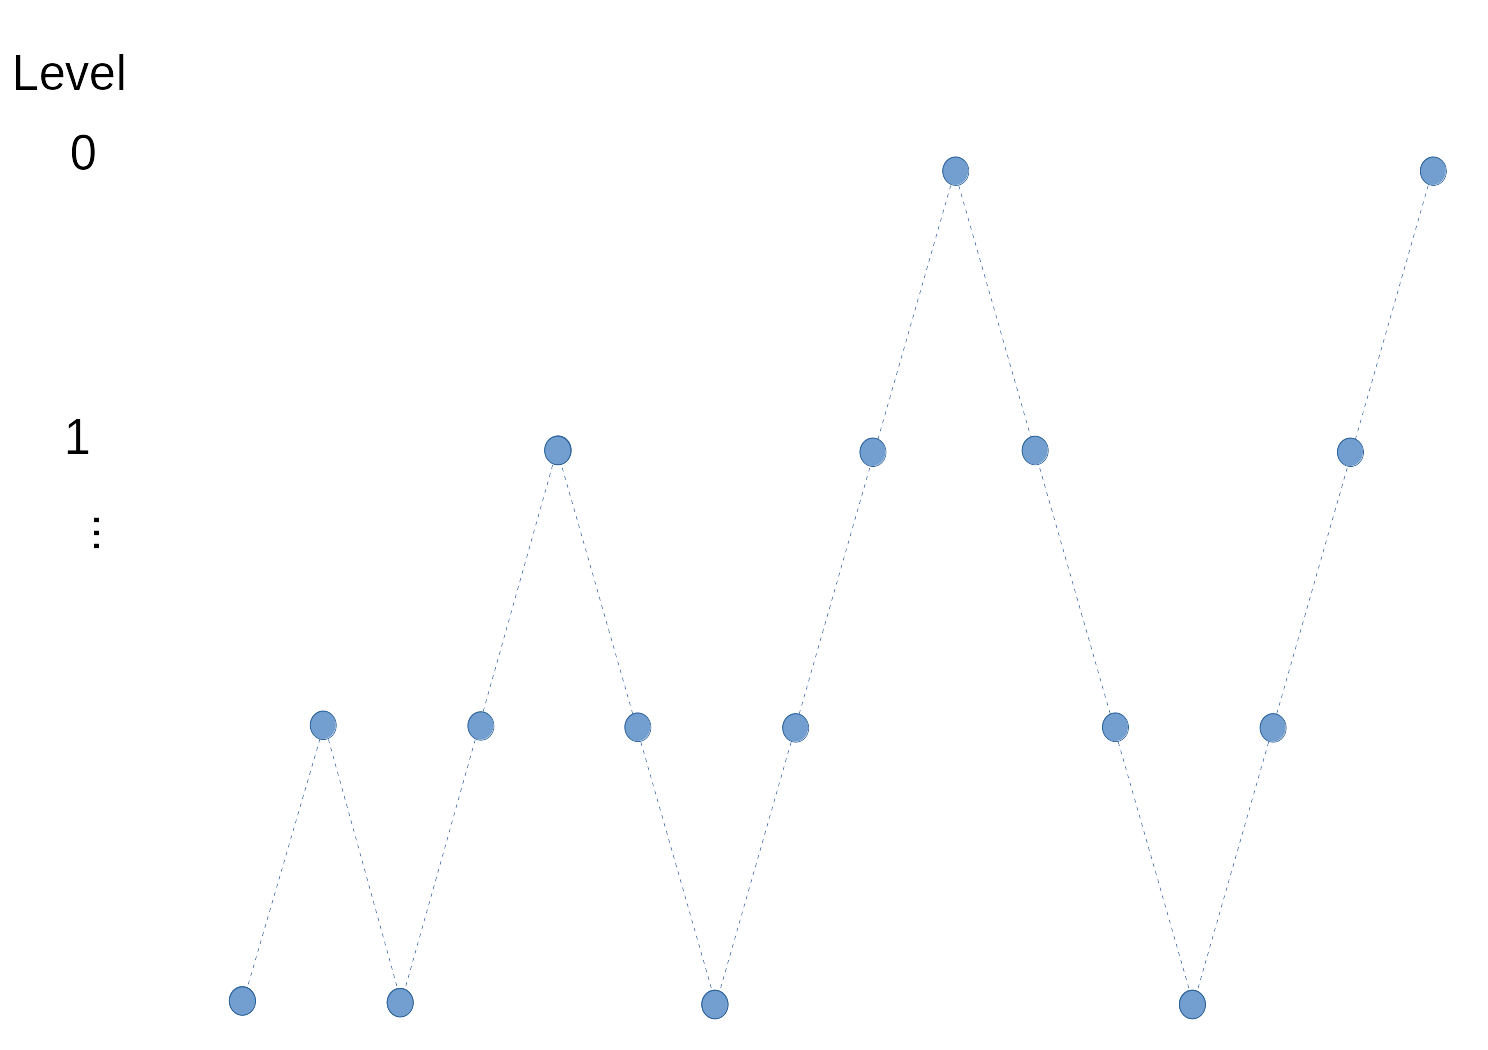
\includegraphics[width=0.7\textwidth]{../figures/FMGcycle}
\end{center}
\end{frame}

% Slide
\begin{frame}{Multigrid cycles}
\begin{block}{Cycle cost and convergence}
\bit
\item Can show that W-cycles and FMG also have $O(N)$ cost
\item V-cycles achieve convergence factors that are independent of $N$
\item Thus V-cycles achieve fixed error reduction with $O(N)$ cost
\item W-cycles similarly achieve fixed error reduction with $O(N)$ cost and can be more robust than V-cycles
\item FMG achieves \emph{discretization accuracy} with $O(N)$ cost!
\eit
\end{block}
\end{frame}

%%%%%%%%%%%%%%%%%%%%%%%%%%%%%%%%%%%%%%%%%%%%%%%%%%%%%%%%%%%%%%%%%%%%%%%%%%%%%%%%

\end{document}

